\documentclass[9pt,a4paper,]{extarticle}

\usepackage{f1000_styles}

\usepackage[pdfborder={0 0 0}]{hyperref}

\usepackage[numbers]{natbib}
\bibliographystyle{unsrtnat}


%% maxwidth is the original width if it is less than linewidth
%% otherwise use linewidth (to make sure the graphics do not exceed the margin)
\makeatletter
\def\maxwidth{ %
  \ifdim\Gin@nat@width>\linewidth
    \linewidth
  \else
    \Gin@nat@width
  \fi
}
\makeatother

\usepackage{color}
\usepackage{fancyvrb}
\newcommand{\VerbBar}{|}
\newcommand{\VERB}{\Verb[commandchars=\\\{\}]}
\DefineVerbatimEnvironment{Highlighting}{Verbatim}{commandchars=\\\{\}}
% Add ',fontsize=\small' for more characters per line
\usepackage{framed}
\definecolor{shadecolor}{RGB}{248,248,248}
\newenvironment{Shaded}{\begin{snugshade}}{\end{snugshade}}
\newcommand{\AlertTok}[1]{\textcolor[rgb]{0.94,0.16,0.16}{#1}}
\newcommand{\AnnotationTok}[1]{\textcolor[rgb]{0.56,0.35,0.01}{\textbf{\textit{#1}}}}
\newcommand{\AttributeTok}[1]{\textcolor[rgb]{0.13,0.29,0.53}{#1}}
\newcommand{\BaseNTok}[1]{\textcolor[rgb]{0.00,0.00,0.81}{#1}}
\newcommand{\BuiltInTok}[1]{#1}
\newcommand{\CharTok}[1]{\textcolor[rgb]{0.31,0.60,0.02}{#1}}
\newcommand{\CommentTok}[1]{\textcolor[rgb]{0.56,0.35,0.01}{\textit{#1}}}
\newcommand{\CommentVarTok}[1]{\textcolor[rgb]{0.56,0.35,0.01}{\textbf{\textit{#1}}}}
\newcommand{\ConstantTok}[1]{\textcolor[rgb]{0.56,0.35,0.01}{#1}}
\newcommand{\ControlFlowTok}[1]{\textcolor[rgb]{0.13,0.29,0.53}{\textbf{#1}}}
\newcommand{\DataTypeTok}[1]{\textcolor[rgb]{0.13,0.29,0.53}{#1}}
\newcommand{\DecValTok}[1]{\textcolor[rgb]{0.00,0.00,0.81}{#1}}
\newcommand{\DocumentationTok}[1]{\textcolor[rgb]{0.56,0.35,0.01}{\textbf{\textit{#1}}}}
\newcommand{\ErrorTok}[1]{\textcolor[rgb]{0.64,0.00,0.00}{\textbf{#1}}}
\newcommand{\ExtensionTok}[1]{#1}
\newcommand{\FloatTok}[1]{\textcolor[rgb]{0.00,0.00,0.81}{#1}}
\newcommand{\FunctionTok}[1]{\textcolor[rgb]{0.13,0.29,0.53}{\textbf{#1}}}
\newcommand{\ImportTok}[1]{#1}
\newcommand{\InformationTok}[1]{\textcolor[rgb]{0.56,0.35,0.01}{\textbf{\textit{#1}}}}
\newcommand{\KeywordTok}[1]{\textcolor[rgb]{0.13,0.29,0.53}{\textbf{#1}}}
\newcommand{\NormalTok}[1]{#1}
\newcommand{\OperatorTok}[1]{\textcolor[rgb]{0.81,0.36,0.00}{\textbf{#1}}}
\newcommand{\OtherTok}[1]{\textcolor[rgb]{0.56,0.35,0.01}{#1}}
\newcommand{\PreprocessorTok}[1]{\textcolor[rgb]{0.56,0.35,0.01}{\textit{#1}}}
\newcommand{\RegionMarkerTok}[1]{#1}
\newcommand{\SpecialCharTok}[1]{\textcolor[rgb]{0.81,0.36,0.00}{\textbf{#1}}}
\newcommand{\SpecialStringTok}[1]{\textcolor[rgb]{0.31,0.60,0.02}{#1}}
\newcommand{\StringTok}[1]{\textcolor[rgb]{0.31,0.60,0.02}{#1}}
\newcommand{\VariableTok}[1]{\textcolor[rgb]{0.00,0.00,0.00}{#1}}
\newcommand{\VerbatimStringTok}[1]{\textcolor[rgb]{0.31,0.60,0.02}{#1}}
\newcommand{\WarningTok}[1]{\textcolor[rgb]{0.56,0.35,0.01}{\textbf{\textit{#1}}}}

% disable code chunks background
%\renewenvironment{Shaded}{}{}

% disable section numbers
\setcounter{secnumdepth}{0}

%% added by MLS, this is not in the F1000 style by default %%

\hypersetup{unicode=true,
            pdftitle={sSNAPPY: an R/Bioconductor package for single-sample directional pathway perturbation analysis},
            pdfkeywords={RNA-seq, pathway enrichment, R package, topology, KEGG, scRNA-seq},
            pdfborder={0 0 0},
            breaklinks=true}

%% End added by MLS %%

\setlength{\parindent}{0pt}
\setlength{\parskip}{6pt plus 2pt minus 1pt}


\usepackage{endfloat}
\usepackage{booktabs}
\usepackage{longtable}
\usepackage{booktabs}
\usepackage{longtable}
\usepackage{array}
\usepackage{multirow}
\usepackage{wrapfig}
\usepackage{float}
\usepackage{colortbl}
\usepackage{pdflscape}
\usepackage{tabu}
\usepackage{threeparttable}
\usepackage{threeparttablex}
\usepackage[normalem]{ulem}
\usepackage{makecell}
\usepackage{xcolor}

\begin{document}
\pagestyle{front}

\title{sSNAPPY: an R/Bioconductor package for single-sample directional pathway perturbation analysis}

\author[1]{Wenjun Liu\thanks{\ttfamily Corresponding Author wenjun.liu@adelaide.edu.au}}
\author[2,3]{Ville-Petteri Mäkinen}
\author[1]{Wayne D. Tilley}
\author[1,4,5]{Stephen M. Pederson}
\affil[1]{Dame Roma Mitchell Cancer Research Laboratories, Adelaide Medical School, Faculty of Health and Medical Sciences, University of Adelaide, Adelaide, Australia}
\affil[2]{Computational Medicine, Faculty of Medicine, University of Oulu, Oulu, Finland}
\affil[3]{Center for Life Course Health Research, Faculty of Medicine, University of Oulu, Oulu, Finland}
\affil[4]{Black Ochre Data Laboratories, Telethon Kids Institute, Adelaide, Australia}
\affil[5]{John Curtin School of Medical Research, Australian National University, Canberra, Australia}

\maketitle
\thispagestyle{front}

\begin{abstract}
A common outcome of analysing RNA-Seq data is the detection of biological pathways with significantly altered activity between the conditions under investigation. Whilst many strategies test for over-representation within pre-defined gene-sets for genes showing changed expression, these analyses typically do not account for gene-gene interactions encoded by pathway topologies, and are not able to directly predict the directional change of pathway activity. To address these issues, we have deloped a single-sample pathway perturbation analysis method \href{https://bioconductor.org/packages/sSNAPPY}{\emph{sSNAPPY}}, now available as an R/Bioconductor package, which leverages pathway topology information to compute pathway perturbation scores, and predicts the direction of change across a set of pathways. Here, we demonstrate the use of \emph{sSNAPPY} by applying the method to public scRNA-seq data, derived from ovarian cancer patient tissues collected before and after chemotherapy. Not only were we able to predict the directions of significant perturbations of pathways discussed in the original study, but \emph{sSNAPPY} was also able to detect significant changes of other biological processes, yielding far greater insight into the response to treatment. \emph{sSNAPPY} represents a novel pathway analysis strategy that takes into consideration of pathway topology to predict impacted biology pathways, both within related samples and across treatment groups. In addition to not relying on the detection of differentially expressed genes, the method and associated R package offer important flexibility and provide powerful visualisation tools.
\end{abstract}

\section*{Keywords}
RNA-seq, pathway enrichment, R package, topology, KEGG, scRNA-seq


\clearpage
\pagestyle{main}

\textbf{R version}: R version 4.3.0 (2023-04-21)

\textbf{Bioconductor version}: 3.17

\textbf{Package}: 1.5.0

\hypertarget{introduction}{%
\section{Introduction}\label{introduction}}

Using pathway enrichment analysis to gain biological insights from gene expression data is a pivotal step in the analysis and interpretation of RNA-seq data, for which numerous methods have been developed (reviewed in \citep{Maleki2020-ur, Mubeen2022-eq}).
Many existing methods tend to view pathways simply as a collection of gene names, as seen in those relying on the detection of differentially expressed genes and applying over-representation analysis (ORA) strategies, and those scoring all genes using functional class scoring (FCS), such as in Gene Set Enrichment Analysis (GSEA) \citep{Subramanian2005-lx}, arguably the most widely-used approach.
However, databases such as the Kyoto Encyclopaedia of Genes and Genomes (KEGG)\citep{OgataKEGGKyotoEncyclopediaa} and WikiPathways\citep{Martens2021} capture not only which genes are implicated in a certain biological process but also their interactions, activating or inhibitory roles, and their relative importance within the pathway, all of which are overlooked in ORA- and FCS-based approaches.

To fully utilise that additional information, the latest generation of pathway analysis approaches include many which are topology-based such as SPIA\citep{Tarca2009}, DEGraph\citep{Jacob2012}, NetGSA\citep{Ma2016} and PRS\citep{Ibrahim2012}, as well as others which explicitly model inter-gene correlations\citep{Wu2012}.
Despite differences in the null hypotheses tested across these approaches, overall, they have demonstrated enhanced sensitivity and specificity due to their abilities to take gene-gene interconnections into account\citep{Nguyen2019-va, Ma2019}.
Nevertheless, most topology-based methods focus only on comparing activities of pathways between two treatment groups and cannot be used to score individual samples (Figure \ref{fig:Figure1}).
However, in heterogenous data where more than one factor may be influencing observations\citep{Hanzelmann2013}, incorporating scoring within paired samples may be desirable and may be able to reveal more nuanced insights.
To address this gap, we present a Single-Sample directioNAl Pathway Perturbation analYsis methodology called \href{https://bioconductor.org/packages/sSNAPPY}{\emph{sSNAPPY}}, available as an R/Bioconductor package.
This article defines how \emph{sSNAPPY} computes changes in gene expression within paired samples, and propagates this through gene-set topologies to predict the perturbation in pathway activities within paired samples, before providing summarised results across an entire dataset (Figure \ref{fig:Figure1}).
The practical usage of the \emph{sSNAPPY} R/Bioconductor package is illustrated through the analysis of a public scRNA-seq dataset using pseudo-bulk strategies.

\begin{figure}

{\centering 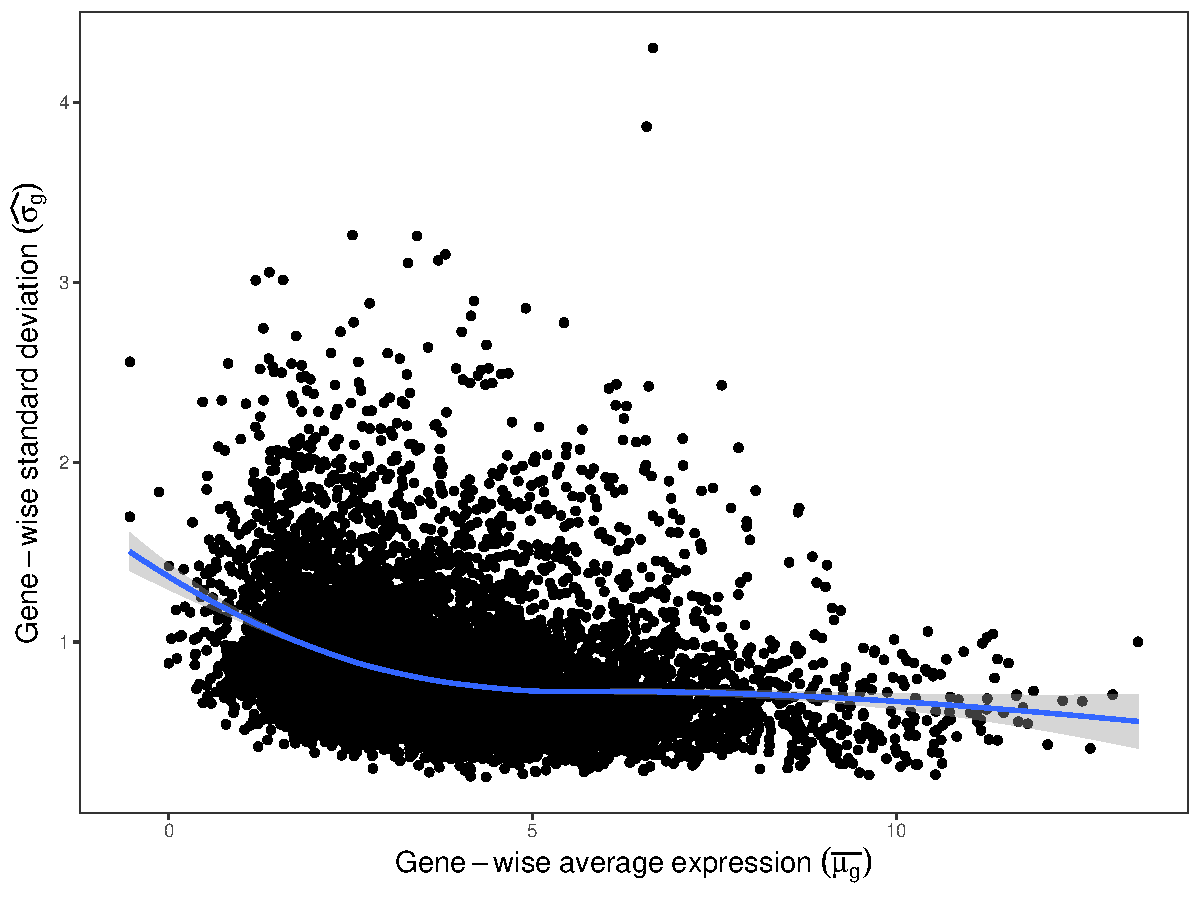
\includegraphics[width=1\linewidth]{sSNAPPY_paper_files/figure-latex/Figure1} 

}

\caption{Schematic illustration of the differences betweeen conventional pathway analysis methods and sSNAPPY. Instead of being limited to treatment-level analyses, \textit{sSNAPPY} allows the detection of pathway perturbation in individual samples by using sample-specific estimates of fold-change instead of experiment-wide estimates. (Created with BioRender.com).}\label{fig:Figure1}
\end{figure}

\hypertarget{methods}{%
\section{Methods}\label{methods}}

\hypertarget{implementation}{%
\subsection{Implementation}\label{implementation}}

\emph{sSNAPPY} is an R package that has been reviewed and published on the open-source bioinformatics software platform \href{https://bioconductor.org/packages/release/bioc/html/*sSNAPPY*.html}{Bioconductor} with all source code available via GitHub.
The methodology itself is topology-based, designed to compute directional, single-sample, pathway perturbation scores in gene expression datasets with a matched-pair, or nested design (eg. samples collected before and after treatment).
This allows for the detection of pathway perturbations within all samples from a treatment group, but also within individual samples.

To run \emph{sSNAPPY}, the only required data is a log-transformed expression matrix (e.g.~logCPM) with matching sample metadata describing treatment groups and the nested structure.
It is assumed that all pre-processing has been performed beforehand, such as the exclusion of low-signal genes or normalisation to minimise technical artefacts like GC-bias.
The first step, performed internally by \emph{sSNAPPY}, is to estimate sample-specific log fold-change (\(\delta_{ghi} = \mu_{ghi} - \mu_{g0i}\)) for a treatment \(h\) across all genes \(g\) within each patient \(i\), by subtracting expression estimates for the baseline samples \(\mu_{g0i}\) from those in the treatment group \(h\).
Here, we gave an example of nesting samples by patients, but \emph{sSNAPPY} could be applied to any data with matched-pair design.
For example, RNA-seq data of treated and untreated cells from several passages, in which case the parameter \(i\) would denote the passages.
It should also be noted that \emph{sSNAPPY} supports any number of treatment/condition levels and the numbers of samples in each treatment group do not have to be identical.
As long as a treated sample is matched to a corresponding control, the sample-specific log fold-changes will be computed for that sample.

Since it has been shown that in RNA-seq data, genes with lower expression tend to have larger variance and larger estimates of change\citep{Law2014}, we utilise a gene-level weighting strategy to de-emphasise logFC estimates for low-abundance genes.
Gene-level weights \(w_g\) are obtained in a treatment-agnostic manner by fitting a loess curve through the relationship between observed gene-level variance (\(\sigma_g\)) and average signal (\(\bar\mu_{g}\))(Figure \ref{fig:Figure2}), and taking the inverse of the loess-predicted variance as the weight \(w_g = a / f(\bar\mu_{g})\), where \(f(\bar\mu_{g})\) is the predicted value from the loess curve and the constant \(a\) ensures \(\sum w_g = 1\).
We then use these weighted estimates of logFC (\(\delta_{ghi}^* = w_g\delta_{ghi}\)) in the calculation of all pathway perturbation scores.

\begin{figure}

{\centering 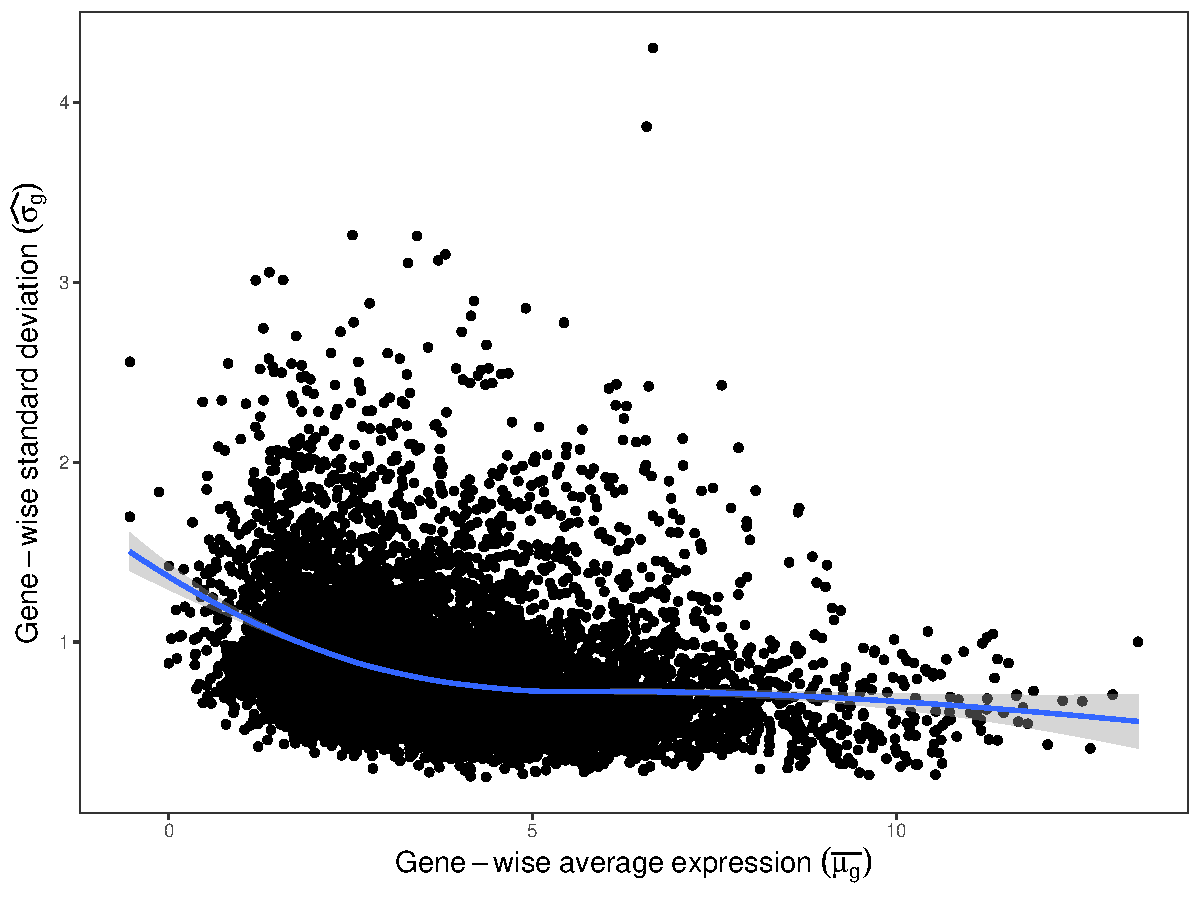
\includegraphics[width=1\linewidth]{sSNAPPY_paper_files/figure-latex/Figure2} 

}

\caption{Gene-wise standard deviations are plotted against the mean logCPM values with mean-variance trend modelled by a loess fit. Genes with low expression values tend to have a larger variance.}\label{fig:Figure2}
\end{figure}

\emph{sSNAPPY} was built upon the group-level topology-based scoring algorithm initially proposed in SPIA\citep{Tarca2009} to propagate genes' changes in expression through pathway topologies to compute a perturbation score for each pathway.
In contrast to SPIA, which requires pre-selection of differentially expressed genes, \emph{sSNAPPY} utilises the full expression matrix.
By modifying the algorithm to incorporate single-sample, weighted estimates of changes in expression we are able to quantify changes in a pathway within a given sample, and then model these across all samples within a treatment group.
Thus, we define the single-sample perturbation score (\(S_{hip}\)) for a given pathway \(p\), patient \(i\) and treatment \(h\):

\[
\begin{aligned}
S_{hip} = \sum_{g \in G_p} \lbrack S_{ghip} - \delta_{ghi}^*\rbrack \text{, where} \\
S_{ghip} = \delta_{ghi}^* + \sum_{g' \in U_{gp}} \beta_{gg'p} \frac{S_{g'hip}}{N_{g'p}} 
\end{aligned}
\]
where:

\begin{itemize}
\item
  \(G_p\) represents the set of genes in pathway \(p\), such that \(g \in G_p\)
\item
  \(S_{ghip}\) is the gene-, treatment- and patient-specific perturbation score for pathway \(p\)
\item
  \(\delta_{ghi}^* = w_g\delta_{ghi}\) is the weighted logFC of gene \(g\) as described above
\item
  \(U_{gp}\) is the subset of \(G_p\) containing only the genes directly upstream of gene \(g\)
\item
  \(\beta_{gg'p}\) is the pair-wise gene-gene interactions\citep{Tarca2009} encoded by the topology matrix for genes \(g\) and \(g'\)
\item
  \(N_{gp}\) is the number of downstream genes from any gene \(g\)
\item
  \(S_{hip}\) is the accumulated pathway perturbation score for pathway \(p\) in treatment \(h\) for patient \(i\)
\end{itemize}

The Bioconductor package graphite\citep{Sales2012} provides functions that can be used to retrieve pathway topologies from a database and convert topology information to adjacency matrices.
In order to streamline this process we have implemented a convenience function, where users only need to provide the name of the desired database and species to retrieve all topology information in the format required by the scoring algorithm with the correct type of gene identifiers (ie. Entrez ID).

To scale the single-sample pathway perturbation scores (\(S_{hip}\)) so they are comparable across pathways and to test for significance of individual scores, null distributions of perturbation scores for each pathway are generated through a sample permutation strategy, retaining the correct correlation structure between genes within a pathway.
In the permutation, all sample labels will be randomly shuffled and assigned to permuted pairs.
Subsequently, permuted single-sample logFCs will be calculated for each pair of permuted samples while the rest of the scoring algorithm remains unchanged.
The median and median absolute deviation (MAD) of the permuted perturbation scores will be calculated within each pathway and used to normalise the raw perturbation scores to robust \(Z\)-scores, which is defined as:

\[
Z_{hip} = \frac{S_{hip} - median_{n \in N}({S_{np}})}{MAD_{n \in N}({S_{np}})}
\]
where \(n\) represents each permuted pairs of samples.
All permuted pairs possible will be constructed in this step by default unless otherwise specified.
In a data with \(I\) total samples, the maximum number of unique permuted pairs \(N\) is \({}^IP_2 = \frac{{I!}}{{(I-2)!}} = I \times (I-1)\).

Following the computation of robust \(Z\)-scores, two-sided \emph{p}-values are derived to assess whether a pathway is significantly perturbed at sample-specific level.
When the sample size is small, the p-values derived from individual robust z-scores should be interpreted with caution.
The MAD and median derived from the permuted scores are more likely to be accurately estimated when the number of permuted scores computed for each pathway is above 100, requiring at least 11 samples.

Apart from assessing whether a pathway's activity changed significantly within an individual sample, users may also be interested in detecting changes at the group-level, which can be performed by modelling scores with regression models, incorporating Smyth's moderated \(t\)-statistic\citep{Smyth_2004} as implemented in \emph{limma}\citep{limma_2015}.
The single-sample nature of \emph{sSNAPPY}'s pathway perturbation scores is particularly helpful for datasets with complex experimental designs or known confounding factors as these can also be incorporated into the final regression models.

\hypertarget{operation}{%
\subsection{Operation}\label{operation}}

The package has been tested on all operating systems, requiring R \textgreater{} 4.3.0, and can be installed using BiocManager as follows.

\begin{Shaded}
\begin{Highlighting}[]
\ControlFlowTok{if}\NormalTok{ (}\SpecialCharTok{!}\FunctionTok{requireNamespace}\NormalTok{(}\StringTok{"BiocManager"}\NormalTok{, }\AttributeTok{quietly =} \ConstantTok{TRUE}\NormalTok{))}
  \FunctionTok{install.packages}\NormalTok{(}\StringTok{"BiocManager"}\NormalTok{)}
\NormalTok{BiocManager}\SpecialCharTok{::}\FunctionTok{install}\NormalTok{(}\StringTok{"sSNAPPY"}\NormalTok{)}
\end{Highlighting}
\end{Shaded}

\hypertarget{use-cases}{%
\section{Use Cases}\label{use-cases}}

\hypertarget{data}{%
\subsection{Data}\label{data}}

To demonstrate the application of \emph{sSNAPPY}, we used pre-processed counts from a publicly available scRNA-seq dataset, retrieved from Gene Expression Omnibus (GEO) with accession code GSE165897.
This dataset consists of 11 high-grade serous ovarian cancer (HGSOC) patients samples taken before and after chemotherapy\citep{Zhang2022}.
\emph{sSNAPPY} was used to re-analyse data from the epithelial cells as they were the primary focus of the original study.
Since \emph{sSNAPPY} was designed for bulk RNA-seq data, counts of epithelial cells from the same samples were first summed into pseudo-bulk profiles, giving rise to a total of 22 samples.
We considered a gene detectable if we observed \textgreater1.5 counts per million in \textgreater11 samples out of 22, representing all samples from a complete treatment group.
11,101 (33.8\%) of the 32,847 annotated genes passed this selection criteria and were included for downstream analyses.
Conditional quantile normalisation\citep{Hansen2012} was then applied to mitigate potential biases introduced by gene length and GC content.
The normalised logCPM matrix of the processed dataset and sample metadata can be downloaded from \href{https://github.com/Wenjun-Liu/F1000_sSNAPPY_manuscript/tree/master/data}{here}.

The following packages are required for this workflow

\begin{Shaded}
\begin{Highlighting}[]
\FunctionTok{library}\NormalTok{(sSNAPPY)}
\FunctionTok{library}\NormalTok{(tidyverse)}
\FunctionTok{library}\NormalTok{(magrittr)}
\FunctionTok{library}\NormalTok{(ggplot2)}
\FunctionTok{library}\NormalTok{(patchwork)}
\FunctionTok{library}\NormalTok{(kableExtra)}
\FunctionTok{library}\NormalTok{(AnnotationHub) }
\FunctionTok{library}\NormalTok{(edgeR)}
\FunctionTok{library}\NormalTok{(patchwork)}
\FunctionTok{library}\NormalTok{(colorspace)}
\end{Highlighting}
\end{Shaded}

Before running the \emph{sSNAPPY} workflow, we need to load our expression matrix and define our sample-level metadata, then download any pathway information.
Firstly we can read in the data, setting the treatment column in the metadata to be a factor.
Importantly, to run \emph{sSNAPPY}, the row names of the expression matrix must be specified as Entrez IDs, for compatibility with pathway databases.
Genes without Entrez IDs were excluded, leaving 10,098 genes in the example expression matrix.

\begin{Shaded}
\begin{Highlighting}[]
\NormalTok{logCPM }\OtherTok{\textless{}{-}} \FunctionTok{read\_tsv}\NormalTok{(here}\SpecialCharTok{::}\FunctionTok{here}\NormalTok{(}\StringTok{"data/logCPM.tsv"}\NormalTok{)) }\SpecialCharTok{\%\textgreater{}\%}
    \FunctionTok{column\_to\_rownames}\NormalTok{(}\StringTok{"entrezid"}\NormalTok{)}
\NormalTok{sample\_meta }\OtherTok{\textless{}{-}} \FunctionTok{read\_tsv}\NormalTok{(here}\SpecialCharTok{::}\FunctionTok{here}\NormalTok{(}\StringTok{"data/sample\_meta.tsv"}\NormalTok{), }\AttributeTok{col\_types =} \StringTok{"cfccncnc"}\NormalTok{)}
\FunctionTok{head}\NormalTok{(sample\_meta)}
\end{Highlighting}
\end{Shaded}

\begin{verbatim}
## # A tibble: 6 x 8
##   sample        treatment patient_id anatomical_location   Age Stage   PFI CRS  
##   <chr>         <fct>     <chr>      <chr>               <dbl> <chr> <dbl> <chr>
## 1 EOC372_treat~ treatmen~ EOC372     Peritoneum             68 IIIC    460 1    
## 2 EOC372_post-~ post-NACT EOC372     Peritoneum             68 IIIC    460 1    
## 3 EOC443_post-~ post-NACT EOC443     Omentum                54 IVA     177 3    
## 4 EOC443_treat~ treatmen~ EOC443     Omentum                54 IVA     177 3    
## 5 EOC540_treat~ treatmen~ EOC540     Omentum                62 IIIC    126 2    
## 6 EOC540_post-~ post-NACT EOC540     Omentum                62 IIIC    126 2
\end{verbatim}

\hypertarget{retrieval-of-pathway-topology}{%
\subsection{Retrieval of Pathway Topology}\label{retrieval-of-pathway-topology}}

Next, pathway topology information needs to be retrieved from a chosen database.
Using KEGG as an example, the retrieved topology information will be stored as a list where each element corresponds to a pathway and the numbers in the matrices encode gene-gene interaction.

\begin{Shaded}
\begin{Highlighting}[]
\NormalTok{gsTopology }\OtherTok{\textless{}{-}} \FunctionTok{retrieve\_topology}\NormalTok{(}\AttributeTok{database =} \StringTok{"kegg"}\NormalTok{, }\AttributeTok{species =} \StringTok{"hsapiens"}\NormalTok{)}
\end{Highlighting}
\end{Shaded}

Instead of downloading the topology matrices of all pathways, it is also possible to provide a restricted set of keywords for a targeted analysis.
In the following we'll use the keywords `metabolism' and `estrogen' to only return a subset of pathways.

\begin{Shaded}
\begin{Highlighting}[]
\CommentTok{\# Only retrieve the topology matrices of metabolism{-} or signalling{-}related pathways}
\NormalTok{gsTopology\_sub }\OtherTok{\textless{}{-}} \FunctionTok{retrieve\_topology}\NormalTok{(}\AttributeTok{database =} \StringTok{"kegg"}\NormalTok{, }\AttributeTok{species =} \StringTok{"hsapiens"}\NormalTok{, }
                                    \AttributeTok{keyword =} \FunctionTok{c}\NormalTok{(}\StringTok{"metabolism"}\NormalTok{, }\StringTok{"estrogen"}\NormalTok{))}
\FunctionTok{names}\NormalTok{(gsTopology\_sub)}
\end{Highlighting}
\end{Shaded}

In addition to working with a single database, users can also choose multiple databases for more comprehensive analyses, albeit with an increased analytic and download time.

\begin{Shaded}
\begin{Highlighting}[]
\NormalTok{gsTopology\_2databases }\OtherTok{\textless{}{-}} \FunctionTok{retrieve\_topology}\NormalTok{(}\AttributeTok{database =} \FunctionTok{c}\NormalTok{(}\StringTok{"kegg"}\NormalTok{, }\StringTok{"wiki"}\NormalTok{), }
                                           \AttributeTok{species =} \StringTok{"hs"}\NormalTok{)}
\end{Highlighting}
\end{Shaded}

\hypertarget{score-single-sample-pathway-perturbation}{%
\subsection{Score Single-Sample Pathway Perturbation}\label{score-single-sample-pathway-perturbation}}

To compute the single-sample expression changes (i.e.~logFC) needed for perturbation scores, samples must be in matched pairs.
For instance, biopsies derived pre- vs post-treatment or untreated vs treated cell lines.
The factor defining the paired structure needs to be passed to the \texttt{weight\_ss\_fc()} function through the \texttt{groupBy} parameter.
In our example dataset, pre- and post-treatment samples are matched by patient IDs.
Additionally, the sample metadata must include the treatment of all samples. The treatment column must be a factor with the reference level set to be the control treatment.

\begin{Shaded}
\begin{Highlighting}[]
\NormalTok{weightedFC }\OtherTok{\textless{}{-}} \FunctionTok{weight\_ss\_fc}\NormalTok{(}\FunctionTok{as.matrix}\NormalTok{(logCPM), }\AttributeTok{metadata =}\NormalTok{ sample\_meta,}
 \AttributeTok{sampleColumn =} \StringTok{"sample"}\NormalTok{, }\AttributeTok{groupBy =} \StringTok{"patient\_id"}\NormalTok{, }\AttributeTok{treatColumn =} \StringTok{"treatment"}\NormalTok{)}
\FunctionTok{glimpse}\NormalTok{(weightedFC)}
\end{Highlighting}
\end{Shaded}

\begin{verbatim}
## List of 2
##  $ weight: num [1:10098] 9.38e-05 1.19e-04 7.63e-05 1.18e-04 1.21e-04 ...
##  $ logFC : num [1:10098, 1:11] -1.52e-05 -2.39e-05 2.00e-04 -1.53e-04 3.84e-05 ...
##   ..- attr(*, "dimnames")=List of 2
##   .. ..$ : chr [1:10098] "ENTREZID:643837" "ENTREZID:26155" "ENTREZID:84069" "ENTREZID:57801" ...
##   .. ..$ : chr [1:11] "EOC372_post-NACT" "EOC443_post-NACT" "EOC540_post-NACT" "EOC3_post-NACT" ...
\end{verbatim}

The output of \texttt{weight\_ss\_fc()} is a \texttt{list} where one element is a matrix of weighted single-sample logFCs (\(\delta_{ghi}^*\)), with rows corresponding to genes and columns to samples, and the other element is the vector of gene-wise weights (\(w_g\)) used to calculate the weighted logFC (\(\delta_{ghi}^*\)), as described above.

The matrix of \(\delta_{ghi}^*\) values are then passed to pathway topologies to compute the gene-wise perturbation scores for all genes included in a pathway, before being summed into a single score for each pathway.
The string \texttt{ENTREZID:} was also added to all row names of the \(\delta_{ghi}^*\) matrix to be compatible with the format pathway topologies were retrieved in.
These gene-wise perturbation scores can also be used in downstream analysis to identify genes playing the most significant roles in each pathway, as will be demonstrated in the visualisation section below.
The pathway-level perturbation scores (\(S_{hip}\)) are returned as a data.frame containing sample and gene-set names.
In the following steps, we first calculate the gene-level contributions to each pathway (\(S_{ghip}\)) using the function \texttt{raw\_gene\_pert()} and then obtain pathway-level summaries using \texttt{pathway\_pert()}.
Pathways with zero perturbation scores across all genes and samples will be dropped at this stage.

\begin{Shaded}
\begin{Highlighting}[]
\NormalTok{genePertScore }\OtherTok{\textless{}{-}} \FunctionTok{raw\_gene\_pert}\NormalTok{(weightedFC}\SpecialCharTok{$}\NormalTok{logFC, gsTopology)}
\NormalTok{ssPertScore }\OtherTok{\textless{}{-}} \FunctionTok{pathway\_pert}\NormalTok{(genePertScore)}
\FunctionTok{head}\NormalTok{(ssPertScore)}
\end{Highlighting}
\end{Shaded}

\begin{verbatim}
##             sample        score                                        gs_name
## 1 EOC372_post-NACT  0.005134216 kegg.EGFR tyrosine kinase inhibitor resistance
## 2 EOC443_post-NACT -0.001959631 kegg.EGFR tyrosine kinase inhibitor resistance
## 3 EOC540_post-NACT -0.006543325 kegg.EGFR tyrosine kinase inhibitor resistance
## 4   EOC3_post-NACT -0.003840943 kegg.EGFR tyrosine kinase inhibitor resistance
## 5  EOC87_post-NACT -0.003917201 kegg.EGFR tyrosine kinase inhibitor resistance
## 6 EOC136_post-NACT -0.008308897 kegg.EGFR tyrosine kinase inhibitor resistance
\end{verbatim}

\hypertarget{sample-permutation-for-normalisation-and-significance-testing}{%
\subsection{Sample Permutation for Normalisation and Significance Testing}\label{sample-permutation-for-normalisation-and-significance-testing}}

The values obtained from each pathway will vary greatly due to the variability in topology structures.
To determine the significance of individual scores and transform scores to ensure they are comparable across pathways, sSNAPPY utilises a sample-permutation strategy to simulate the null distributions of perturbation scores.
Since sample labels will be permuted randomly to put samples into pairs, sample metadata is not required by the \texttt{generate\_permuted\ \_scores()} function.
All the possible random pairs between samples will be constructed by default, unless otherwise specified by the \texttt{NB} parameter.
In this example dataset with a total of 22 samples, 462 (i.e.~22 \(\times\) 21) permuted scores will be computed for each pathway.,

\begin{Shaded}
\begin{Highlighting}[]
\FunctionTok{set.seed}\NormalTok{(}\DecValTok{123}\NormalTok{)}
\NormalTok{permutedScore }\OtherTok{\textless{}{-}} \FunctionTok{generate\_permuted\_scores}\NormalTok{(}
    \FunctionTok{as.matrix}\NormalTok{(logCPM), }\AttributeTok{gsTopology =}\NormalTok{ gsTopology, }\AttributeTok{weight =}\NormalTok{ weightedFC}\SpecialCharTok{$}\NormalTok{weight}
\NormalTok{)}
\end{Highlighting}
\end{Shaded}

Apart from pathways whose permuted perturbation scores are all zero, the rest of the pathways' empirical distributions should be approximately normally distributed with means equal to zero.
To demonstrate that, we randomly selected 6 pathways and visualised the permuted perturbation scores as boxplots (Figure \ref{fig:Figure3}).

\begin{Shaded}
\begin{Highlighting}[]
\FunctionTok{set.seed}\NormalTok{(}\DecValTok{234}\NormalTok{)}
\NormalTok{permutedScore }\SpecialCharTok{\%\textgreater{}\%}
    \FunctionTok{keep}\NormalTok{(}\SpecialCharTok{\textasciitilde{}}\FunctionTok{all}\NormalTok{(.}\SpecialCharTok{!=}\DecValTok{0}\NormalTok{)) }\SpecialCharTok{\%\textgreater{}\%}
\NormalTok{    .[}\FunctionTok{sample}\NormalTok{(}\FunctionTok{seq\_along}\NormalTok{(.), }\DecValTok{6}\NormalTok{)] }\SpecialCharTok{\%\textgreater{}\%}
    \FunctionTok{as.data.frame}\NormalTok{() }\SpecialCharTok{\%\textgreater{}\%}
    \FunctionTok{pivot\_longer}\NormalTok{(}
      \AttributeTok{cols =} \FunctionTok{everything}\NormalTok{(), }\AttributeTok{names\_to =} \StringTok{"gs\_name"}\NormalTok{, }\AttributeTok{values\_to =} \StringTok{"score"}
\NormalTok{    ) }\SpecialCharTok{\%\textgreater{}\%}
    \FunctionTok{mutate}\NormalTok{(}
        \AttributeTok{gs\_name =} \FunctionTok{str\_replace\_all}\NormalTok{(gs\_name, }\StringTok{"}\SpecialCharTok{\textbackslash{}\textbackslash{}}\StringTok{."}\NormalTok{, }\StringTok{" "}\NormalTok{),}
        \AttributeTok{gs\_name =} \FunctionTok{str\_remove\_all}\NormalTok{(gs\_name, }\StringTok{"kegg "}\NormalTok{)}
\NormalTok{    ) }\SpecialCharTok{\%\textgreater{}\%}
    \FunctionTok{ggplot}\NormalTok{(}\FunctionTok{aes}\NormalTok{(gs\_name, score, }\AttributeTok{fill =}\NormalTok{ gs\_name)) }\SpecialCharTok{+}
    \FunctionTok{geom\_boxplot}\NormalTok{() }\SpecialCharTok{+}
    \FunctionTok{scale\_x\_discrete}\NormalTok{(}\AttributeTok{labels =} \ControlFlowTok{function}\NormalTok{(x) }\FunctionTok{str\_wrap}\NormalTok{(x, }\AttributeTok{width =} \DecValTok{10}\NormalTok{)) }\SpecialCharTok{+}
    \FunctionTok{scale\_fill\_discrete}\NormalTok{(}\AttributeTok{name =} \StringTok{"Gene{-}set Name"}\NormalTok{) }\SpecialCharTok{+} 
    \FunctionTok{labs}\NormalTok{(}\AttributeTok{x =} \StringTok{"Pathway"}\NormalTok{, }\AttributeTok{y =} \StringTok{"Permuted Perturbation Score"}\NormalTok{) }\SpecialCharTok{+}
    \FunctionTok{theme\_bw}\NormalTok{() }\SpecialCharTok{+} 
    \FunctionTok{theme}\NormalTok{(}
      \AttributeTok{legend.position =} \StringTok{"none"}\NormalTok{, }
      \AttributeTok{axis.title =} \FunctionTok{element\_text}\NormalTok{(}\AttributeTok{size =} \DecValTok{16}\NormalTok{), }
      \AttributeTok{axis.text =} \FunctionTok{element\_text}\NormalTok{(}\AttributeTok{size =} \DecValTok{14}\NormalTok{)}
\NormalTok{    )}
\end{Highlighting}
\end{Shaded}

\begin{figure}

{\centering 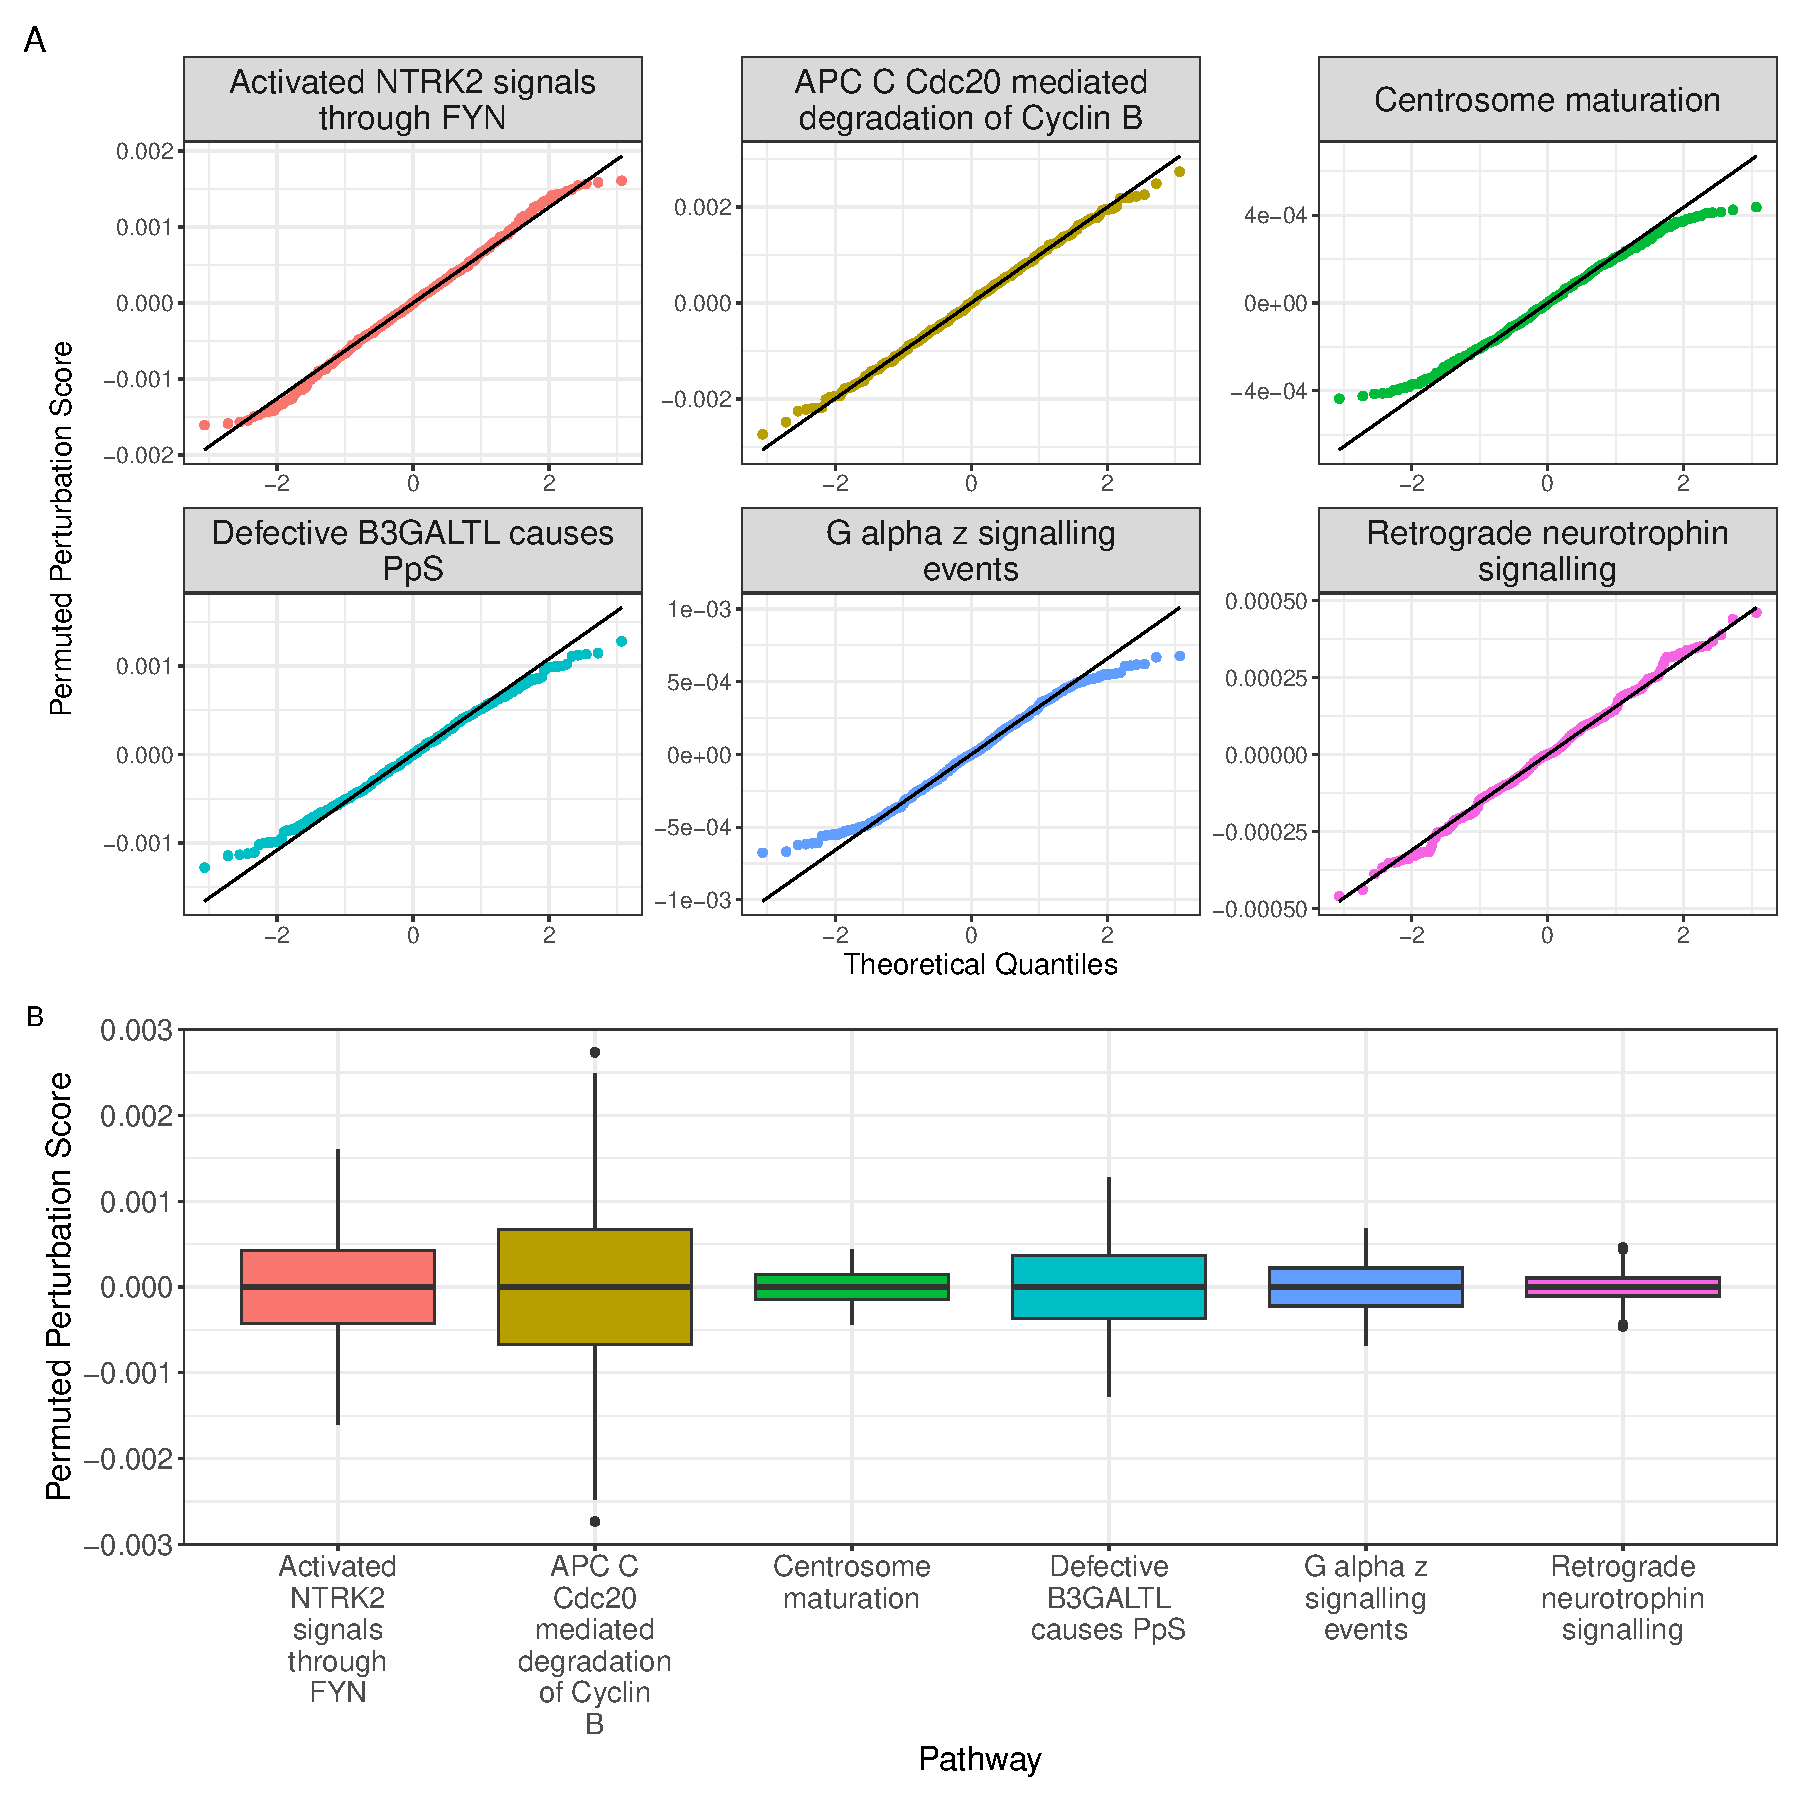
\includegraphics[width=1\linewidth]{sSNAPPY_paper_files/figure-latex/Figure3-1} 

}

\caption{Permuted perturbation scores of six randomly selected pathways. All sampled empirical distributions are approximately normally distributed with a mean of zero.}\label{fig:Figure3}
\end{figure}

Permuted distributions are used to convert each pathway-level score into a scaled robust \(Z\)-score using the function \texttt{normalise\_by\_permu()}.
Robust Z-scores can in turn be transformed into two-sided p-values and corrected for multiple testing using any of the available methods, and returning the FDR adjusted values by default.
In our brief example data, no pathways would be considered as significantly perturbed at the single-sample level using an FDR adjustment with \(\alpha\) = 0.05.

\begin{Shaded}
\begin{Highlighting}[]
\NormalTok{normalisedScores }\OtherTok{\textless{}{-}} \FunctionTok{normalise\_by\_permu}\NormalTok{(permutedScore, ssPertScore, }
                                       \AttributeTok{sortBy =} \StringTok{"pvalue"}\NormalTok{)}
\FunctionTok{head}\NormalTok{(normalisedScores)}
\end{Highlighting}
\end{Shaded}

\begin{verbatim}
##               MAD MEDIAN                                       gs_name
## 388  0.0274269216      0             kegg.Epstein-Barr virus infection
## 417  0.0002129708      0               kegg.Autoimmune thyroid disease
## 421  0.0002129708      0                      kegg.Allograft rejection
## 287  0.0142815123      0               kegg.JAK-STAT signaling pathway
## 1142 0.0034839083      0 kegg.C-type lectin receptor signaling pathway
## 505  0.0099700991      0                kegg.Th17 cell differentiation
##                sample         score   robustZ      pvalue adjPvalue
## 388  EOC136_post-NACT -0.0817379496 -2.980209 0.002880521 0.2427042
## 417  EOC136_post-NACT -0.0006237555 -2.928831 0.003402395 0.2427042
## 421  EOC136_post-NACT -0.0006237555 -2.928831 0.003402395 0.2427042
## 287  EOC136_post-NACT -0.0366880290 -2.568918 0.010201670 0.5457893
## 1142 EOC349_post-NACT  0.0085037555  2.440867 0.014652066 0.9834071
## 505  EOC153_post-NACT  0.0238610587  2.393262 0.016699314 0.7836214
\end{verbatim}

A key question of interest in this dataset is to identify which biological processes were impacted by chemotherapy across the entire group of patients.
Using the sample-level output obtained above, we can explore this by applying t-tests or regression models across all samples.
In order to minimise spurious results, Smyth's moderated t-statistics\citep{Smyth_2004} are able to be applied across the complete dataset.
Given that we have robust Z-score, a constant variance was assumed across all pathways.
To perform this analysis, the robust Z-scores were converted to a matrix, and the standard limma methodologies was used with variance set to be constant.
For our use case here, no design matrix is required and a simple t-test is appropriate.

\begin{Shaded}
\begin{Highlighting}[]
\NormalTok{z\_matrix }\OtherTok{\textless{}{-}}\NormalTok{ normalisedScores }\SpecialCharTok{\%\textgreater{}\%}
\NormalTok{  dplyr}\SpecialCharTok{::}\FunctionTok{select}\NormalTok{(robustZ, gs\_name, sample) }\SpecialCharTok{\%\textgreater{}\%}
  \FunctionTok{pivot\_wider}\NormalTok{(}\AttributeTok{names\_from =} \StringTok{"sample"}\NormalTok{, }\AttributeTok{values\_from =} \StringTok{"robustZ"}\NormalTok{) }\SpecialCharTok{\%\textgreater{}\%}
  \FunctionTok{column\_to\_rownames}\NormalTok{(}\StringTok{"gs\_name"}\NormalTok{) }\SpecialCharTok{\%\textgreater{}\%}
  \FunctionTok{as.matrix}\NormalTok{()}
\NormalTok{z\_fits }\OtherTok{\textless{}{-}} \FunctionTok{lmFit}\NormalTok{(z\_matrix, }\AttributeTok{design =} \FunctionTok{rep}\NormalTok{(}\DecValTok{1}\NormalTok{, }\FunctionTok{ncol}\NormalTok{(z\_matrix))) }\SpecialCharTok{\%\textgreater{}\%} 
  \FunctionTok{eBayes}\NormalTok{(}\AttributeTok{trend =} \ConstantTok{FALSE}\NormalTok{)}
\NormalTok{top\_table }\OtherTok{\textless{}{-}} \FunctionTok{topTable}\NormalTok{(z\_fits, }\AttributeTok{number =} \ConstantTok{Inf}\NormalTok{) }\SpecialCharTok{\%\textgreater{}\%}
  \FunctionTok{as\_tibble}\NormalTok{(}\AttributeTok{rownames =} \StringTok{"gs\_name"}\NormalTok{)}
\end{Highlighting}
\end{Shaded}

Pathways with an FDR \textless{} 0.05 in the moderated t-test were considered to be significantly perturbed at the group level.
8 out of the 315 tested KEGG pathways passed the selection threshold (Table \ref{tab:Table1}).

\begin{Shaded}
\begin{Highlighting}[]
\NormalTok{table1 }\OtherTok{\textless{}{-}}\NormalTok{ top\_table }\SpecialCharTok{\%\textgreater{}\%}
\NormalTok{  dplyr}\SpecialCharTok{::}\FunctionTok{filter}\NormalTok{(adj.P.Val }\SpecialCharTok{\textless{}} \FloatTok{0.05}\NormalTok{) }\SpecialCharTok{\%\textgreater{}\%} 
  \FunctionTok{mutate}\NormalTok{(}
    \AttributeTok{Direction =} \FunctionTok{ifelse}\NormalTok{(logFC }\SpecialCharTok{\textless{}} \DecValTok{0}\NormalTok{, }\StringTok{"Inhibited"}\NormalTok{, }\StringTok{"Activated"}\NormalTok{), }
    \AttributeTok{gs\_name =} \FunctionTok{str\_remove\_all}\NormalTok{(gs\_name, }\StringTok{"kegg."}\NormalTok{)}
\NormalTok{  ) }\SpecialCharTok{\%\textgreater{}\%}
\NormalTok{  dplyr}\SpecialCharTok{::}\FunctionTok{select}\NormalTok{(}
    \AttributeTok{Pathway =}\NormalTok{ gs\_name, }\AttributeTok{Change =}\NormalTok{ logFC,  P.Value, }\AttributeTok{FDR =}\NormalTok{ adj.P.Val, Direction}
\NormalTok{  )}
\end{Highlighting}
\end{Shaded}

\begin{table}

\caption{\label{tab:Table1}Significantly impacted KEGG pathways identified among post-chemotherapy samples using sSNAPPY}
\centering
\resizebox{\linewidth}{!}{
\begin{tabular}[t]{lrrrl}
\toprule
Pathway & Change & P.Value & FDR & Direction\\
\midrule
\cellcolor{gray!6}{AMPK signaling pathway} & \cellcolor{gray!6}{0.86} & \cellcolor{gray!6}{1.6e-05} & \cellcolor{gray!6}{0.0035} & \cellcolor{gray!6}{Activated}\\
Progesterone-mediated oocyte maturation & -0.77 & 2.9e-04 & 0.0220 & Inhibited\\
\cellcolor{gray!6}{p53 signaling pathway} & \cellcolor{gray!6}{0.86} & \cellcolor{gray!6}{3.1e-04} & \cellcolor{gray!6}{0.0220} & \cellcolor{gray!6}{Activated}\\
Pathogenic Escherichia coli infection & 0.66 & 5.1e-04 & 0.0272 & Activated\\
\cellcolor{gray!6}{Cellular senescence} & \cellcolor{gray!6}{0.71} & \cellcolor{gray!6}{7.8e-04} & \cellcolor{gray!6}{0.0334} & \cellcolor{gray!6}{Activated}\\
\addlinespace
Parathyroid hormone synthesis, secretion and action & 0.65 & 1.1e-03 & 0.0386 & Activated\\
\cellcolor{gray!6}{Yersinia infection} & \cellcolor{gray!6}{0.64} & \cellcolor{gray!6}{1.8e-03} & \cellcolor{gray!6}{0.0496} & \cellcolor{gray!6}{Activated}\\
Toxoplasmosis & 0.65 & 1.9e-03 & 0.0496 & Activated\\
\bottomrule
\end{tabular}}
\end{table}

For enrichment analysis in the original study\citep{Zhang2022}, unsupervised clustering was performed on all cells labelled as cancer cells.
Clusters were then annotated manually by performing pathway enrichment testing on cluster marker genes.
Two clusters, associated with proliferative DNA repair signatures and stress-related markers, contained significantly higher numbers of post-chemotherapy cells than pre-treatment ones\citep{Zhang2022}.
The representative pathways enriched in the stress-associated cluster were \emph{IL6-mediated signaling events}, \emph{TNF signaling pathway}, and \emph{cellular responses to stress}, characterized by marker genes \emph{JUN}, \emph{FOS}, \emph{IL6}, \emph{TNF}, \emph{CXCR4}, \emph{SNAI1}, \emph{VIM}, \emph{GADD45B}, and \emph{MCL1.}
Among the stress-related marker genes reported, 5 of them(\emph{FOS}, \emph{GADD45B}, \emph{IL6}, \emph{JUN}, and \emph{TNF}) were implicated in pathways that were considered to be significantly impacted by sSNAPPY.
The other post-chemotherapy cell dominated cluster in the original study was enriched for pathways associated with cell proliferation and DNA repair, such as the Cell cycle, DNA repair, Homology directed repair (HDR) through homologous recombination, and Fanconi anaemia pathway.
A key gene involved in those pathways was \emph{CHEK1}, which was also found in significantly perturbed pathways detected by sSNAPPY: the p53 signaling pathway and Cellular senescence pathway.

Apart from considering all treated samples as biological replicates, users may elect to perform an analysis incorporating other phenotypic traits that affect patients' responses to chemotherapy, such as disease stages or tumour grades.
To do that through the moderated t-statistic strategy and extend the above analysis, all that is required is an appropriate design matrix in the \texttt{lmFit} step, or subsetting the samples accordingly

\hypertarget{visualising-perturbed-pathways-as-networks}{%
\subsection{Visualising Perturbed Pathways as Networks}\label{visualising-perturbed-pathways-as-networks}}

A valuable feature of sSNAPPY is the provision of various visualisation functions to assist in the interpretation of results.
Biological pathways are not independent of each other with many genes playing a role across multiple pathways, and as such, visualising pathway analysis results as a network can be a powerful way to intuitively summarise the results and facilitate interpretation of the underlying biology.
The \texttt{plot\_gs\_network()} function allows users to easily convert a list of perturbed biological pathways to a network where edges between pathway nodes represent overlapping genes.
Defined by the colorBy parameter, pathway nodes can be coloured by either the pathways' predicted direction of changes or the significance levels (Figure \ref{fig:Figure4}).
The returned plot is a ggplot2 \citep{Wickham2009} object, meaning that components of the plotting theme and other parameters can be customized as for any other ggplot2 objects.

First we should obtain a subset of pathways to visualise.
In the following example, the most highly ranked pathways were inspected, which involved three steps to prepare the data: 1) rename the logFC column to reflect the true meaning of the value and, 2) create a categorical variable with the pathway status, 3) transform the p-values for simpler visualisation.

\begin{Shaded}
\begin{Highlighting}[]
\NormalTok{sigPathway }\OtherTok{\textless{}{-}}\NormalTok{ top\_table }\SpecialCharTok{\%\textgreater{}\%}
\NormalTok{  dplyr}\SpecialCharTok{::}\FunctionTok{filter}\NormalTok{(adj.P.Val }\SpecialCharTok{\textless{}} \FloatTok{0.05}\NormalTok{) }\SpecialCharTok{\%\textgreater{}\%} 
\NormalTok{  dplyr}\SpecialCharTok{::}\FunctionTok{rename}\NormalTok{(}\AttributeTok{Z =}\NormalTok{ logFC) }\SpecialCharTok{\%\textgreater{}\%} 
  \FunctionTok{mutate}\NormalTok{(}
    \AttributeTok{status =} \FunctionTok{ifelse}\NormalTok{(}
\NormalTok{        Z }\SpecialCharTok{\textgreater{}} \DecValTok{0}\NormalTok{, }\StringTok{"Activated"}\NormalTok{, }\StringTok{"Inhibited"}
\NormalTok{    ),}
    \AttributeTok{status =} \FunctionTok{as.factor}\NormalTok{(status),}
    \StringTok{\textasciigrave{}}\AttributeTok{{-}log10(p)}\StringTok{\textasciigrave{}} \OtherTok{=} \SpecialCharTok{{-}}\FunctionTok{log10}\NormalTok{(P.Value)}
\NormalTok{  )}
\end{Highlighting}
\end{Shaded}

\begin{Shaded}
\begin{Highlighting}[]
\FunctionTok{set.seed}\NormalTok{(}\DecValTok{123}\NormalTok{)}
\CommentTok{\# Plot the network structure}
\NormalTok{p1 }\OtherTok{\textless{}{-}} \FunctionTok{plot\_gs\_network}\NormalTok{(}
  \AttributeTok{normalisedScores =}\NormalTok{ sigPathway, }\AttributeTok{gsTopology =}\NormalTok{ gsTopology, }\AttributeTok{colorBy =} \StringTok{"status"}
\NormalTok{) }\SpecialCharTok{+}
  \FunctionTok{scale\_colour\_manual}\NormalTok{(}\AttributeTok{values =} \FunctionTok{c}\NormalTok{(}\StringTok{"red"}\NormalTok{, }\StringTok{"blue"}\NormalTok{, }\StringTok{"grey30"}\NormalTok{)) }\SpecialCharTok{+}
  \FunctionTok{theme\_void}\NormalTok{()}
\FunctionTok{set.seed}\NormalTok{(}\DecValTok{123}\NormalTok{)}
\NormalTok{p2 }\OtherTok{\textless{}{-}} \FunctionTok{plot\_gs\_network}\NormalTok{(}
  \AttributeTok{normalisedScores =}\NormalTok{ sigPathway,}
  \AttributeTok{gsTopology =}\NormalTok{ gsTopology, }
  \AttributeTok{colorBy  =} \StringTok{"{-}log10(p)"}\NormalTok{, }
  \AttributeTok{color\_lg\_title =} \FunctionTok{expression}\NormalTok{(}\FunctionTok{paste}\NormalTok{(}\SpecialCharTok{{-}}\NormalTok{log[}\DecValTok{10}\NormalTok{], }\StringTok{"p"}\NormalTok{))}
\NormalTok{) }\SpecialCharTok{+}
  \FunctionTok{scale\_colour\_viridis\_c}\NormalTok{() }\SpecialCharTok{+}
  \FunctionTok{theme\_void}\NormalTok{()}
\NormalTok{p1 }\SpecialCharTok{+}\NormalTok{ p2 }\SpecialCharTok{+} \FunctionTok{plot\_annotation}\NormalTok{(}\AttributeTok{tag\_levels =} \StringTok{"A"}\NormalTok{) }
\end{Highlighting}
\end{Shaded}

\begin{figure}

{\centering 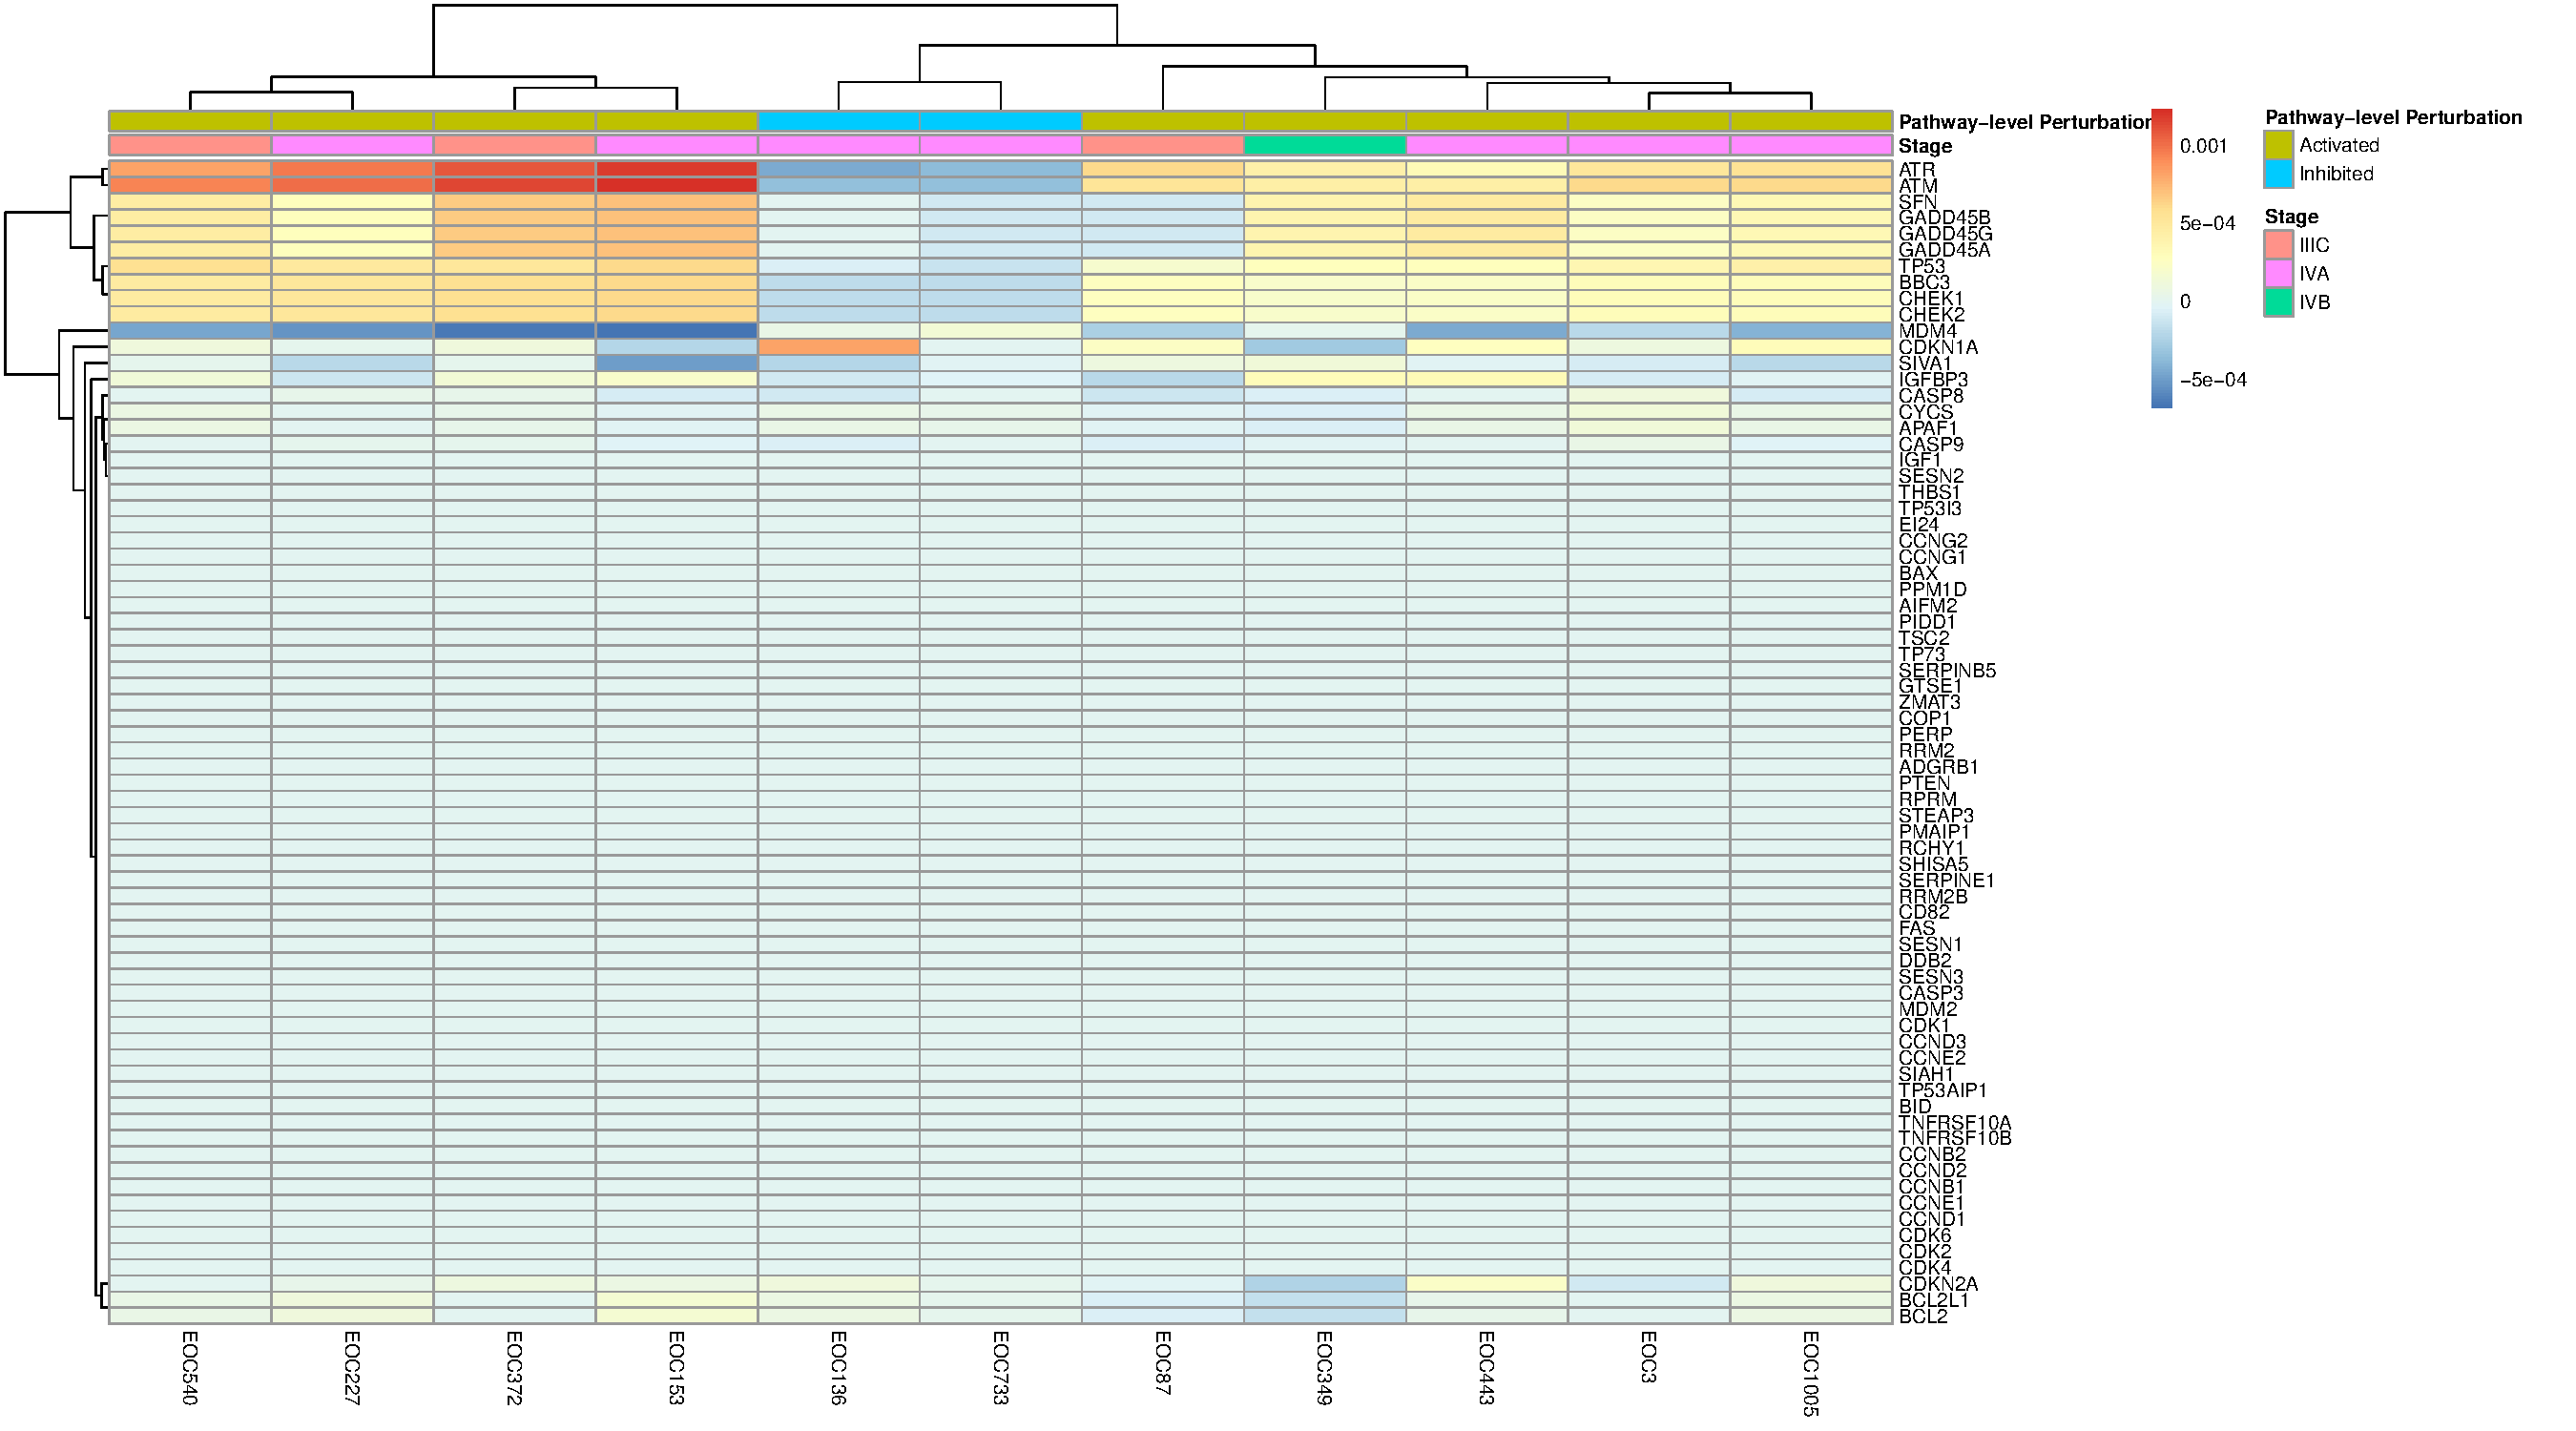
\includegraphics[width=1\linewidth]{sSNAPPY_paper_files/figure-latex/Figure4-1} 

}

\caption{Significantly perturbed KEGG pathways identified among post-chemotherapy samples using sSNAPPY, colored by (A) pathways’ predicted direction of changes and (B) pathways’ -log10(p-values). Pathways with a FDR < 0.05 in the moderated t-test were included.}\label{fig:Figure4}
\end{figure}

By examining the network structure, we can see that many of the highly connected pathways playing a central role in the network are infection-related (Figure \ref{fig:Figure4}).
To summarise related pathways and further enable interpretation, we can apply community detection\citep{Newman2004} in order to group related pathways into `communities'.
sSNAPPY's \texttt{plot\_community()} function is a one-stop shop for applying a community detection algorithm of the user's choice to the network structure and annotating identified communities by the most common pathway category, denoting the main biological processes perturbed in that community.
The most recent categories for KEGG pathways were curated from the \href{https://www.genome.jp/kegg/pathway.html}{KEGG website} and included as part of sSNAPPY.
Annotation of KEGG pathway communities is automatically completed by calling the in-built data object.
Analyses involving other pathway databases will require user-provided pathway categories.
In the current dataset, the Louvain method was applied to the network of biological pathways and revealed two primary communities, where one was annotated to be cell cycle and endocrine system related and the other one was most closely related to infectious diseases (Figure \ref{fig:Figure5}).

\begin{Shaded}
\begin{Highlighting}[]
\FunctionTok{set.seed}\NormalTok{(}\DecValTok{123}\NormalTok{)}
\FunctionTok{plot\_community}\NormalTok{(}
    \AttributeTok{normalisedScores =}\NormalTok{ sigPathway,}
    \AttributeTok{gsTopology =}\NormalTok{ gsTopology, }
    \AttributeTok{colorBy =} \StringTok{"status"}
    
\NormalTok{) }\SpecialCharTok{+}
    \FunctionTok{scale\_colour\_manual}\NormalTok{(}\AttributeTok{values =} \FunctionTok{c}\NormalTok{(}\StringTok{"red"}\NormalTok{, }\StringTok{"blue"}\NormalTok{)) }\SpecialCharTok{+}
    \FunctionTok{scale\_fill\_viridis\_d}\NormalTok{() }\SpecialCharTok{+}
    \FunctionTok{scale\_x\_continuous}\NormalTok{(}\AttributeTok{expand =} \FunctionTok{expansion}\NormalTok{(}\FloatTok{0.25}\NormalTok{)) }\SpecialCharTok{+}
    \FunctionTok{scale\_y\_continuous}\NormalTok{(}\AttributeTok{expand =} \FunctionTok{expansion}\NormalTok{(}\FloatTok{0.25}\NormalTok{)) }\SpecialCharTok{+}
    \FunctionTok{theme\_void}\NormalTok{() }
\end{Highlighting}
\end{Shaded}

\begin{figure}

{\centering 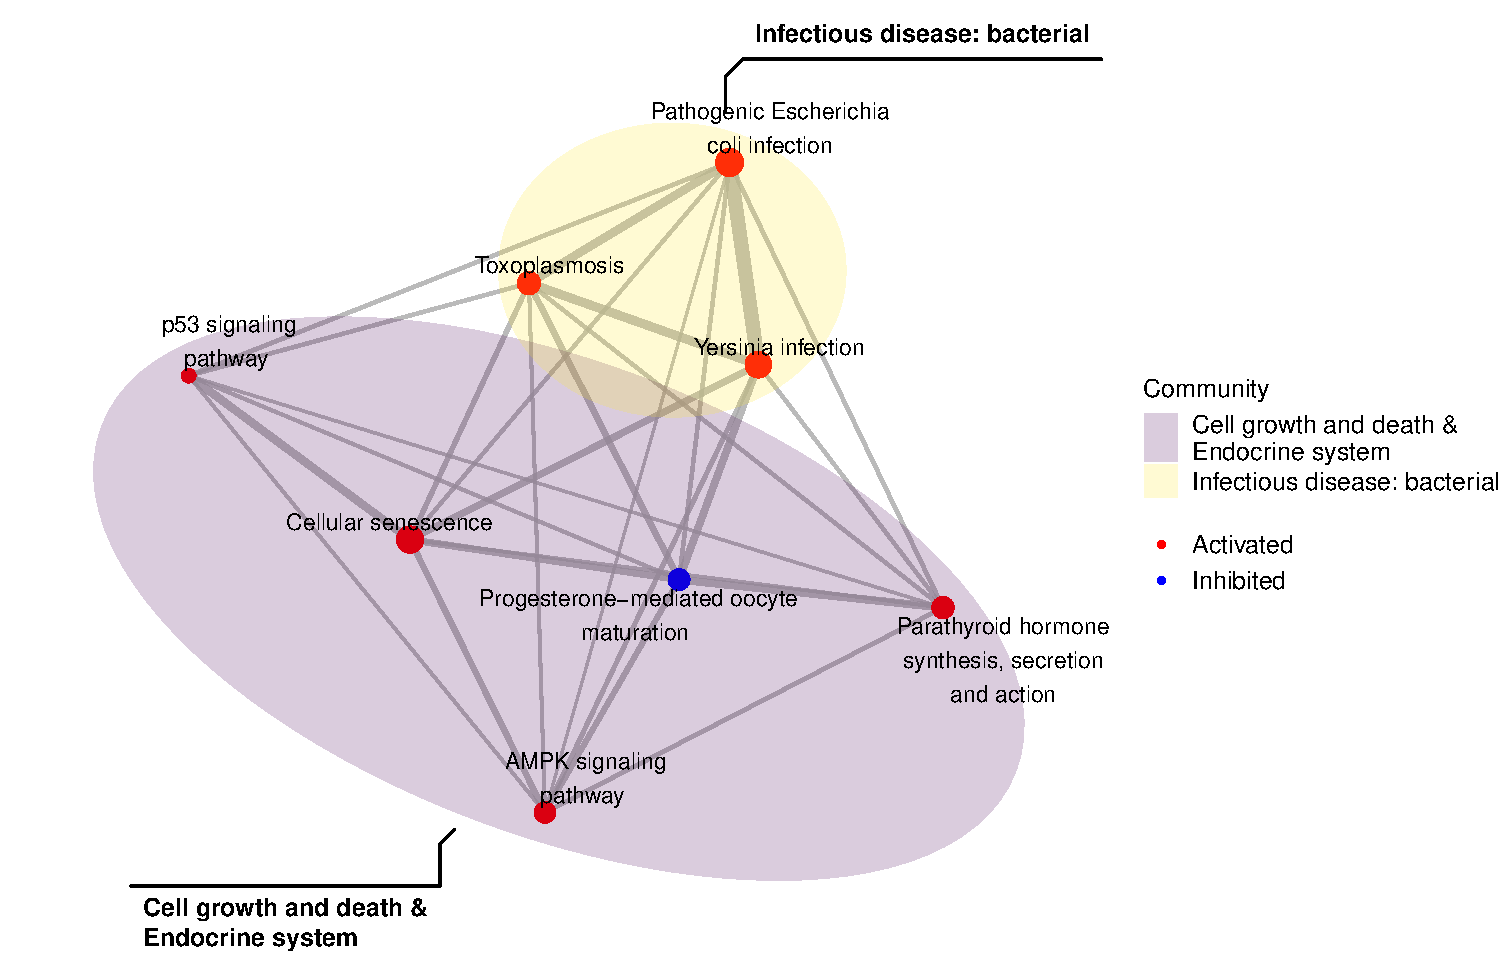
\includegraphics[width=0.8\linewidth]{sSNAPPY_paper_files/figure-latex/Figure5-1} 

}

\caption{Significantly perturbed KEGG pathways identified among post-chemotherapy samples using sSNAPPY, colored by community structures detected through the louvain algorithm. The main biological processes perturbed by the chemo-therapy were shown.}\label{fig:Figure5}
\end{figure}

A key advantage of sSNAPPY is that it does not require the prior identification of differentially expressed genes, as this is not always possible in clinical datasets.
However, knowing which genes are implicated in the perturbation of pathways, particularly those which influence multiple pathways, can provide valuable insights for hypotheses generation about underlying biological mechanisms.
Therefore, sSNAPPY provides another visualisation feature called \texttt{plot\_gs2gene}, which enables the inclusion of select genes from each pathway using network structures.
Users can provide a vector of fold-change estimates to visualise genes within pathways, showing their estimated change in expression.
As pathways often include hundreds of genes, it is recommended to filter for genes most likely to be playing a significant role.
In this example dataset, only genes within the top 500 when ranking by the magnitude of the mean log fold-change were included (Figure \ref{fig:Figure6}).
An alternative strategy will be to select genes based on test-statistics, however, this decision is up to the individual researcher.

\begin{Shaded}
\begin{Highlighting}[]
\NormalTok{meanFC }\OtherTok{\textless{}{-}} \FunctionTok{rowMeans}\NormalTok{(weightedFC}\SpecialCharTok{$}\NormalTok{logFC) }\SpecialCharTok{/}\NormalTok{ weightedFC}\SpecialCharTok{$}\NormalTok{weight}
\NormalTok{top500 }\OtherTok{\textless{}{-}} \FunctionTok{rank}\NormalTok{(}\DecValTok{1}\SpecialCharTok{/}\FunctionTok{abs}\NormalTok{(meanFC)) }\SpecialCharTok{\textless{}=} \DecValTok{500}
\NormalTok{dirFC }\OtherTok{\textless{}{-}} \FunctionTok{ifelse}\NormalTok{(meanFC }\SpecialCharTok{\textgreater{}} \DecValTok{0}\NormalTok{, }\StringTok{"Up{-}Regulated"}\NormalTok{, }\StringTok{"Down{-}Regulated"}\NormalTok{)}
\end{Highlighting}
\end{Shaded}

Since KEGG pathway topologies were retrieved using EntrezIDs, users can provide a data.frame mapping Entrez IDs to their chosen identifiers, such as gene names, through the mapEntrezID parameter to make the visualisations more informative.
A data.frame converting Entrez IDs to ensemble gene names was derived from the Ensembl Release 101\citep{Ensembl2022} and has been made available as part of the package.

\begin{Shaded}
\begin{Highlighting}[]
\FunctionTok{load}\NormalTok{(}\FunctionTok{system.file}\NormalTok{(}\StringTok{"extdata"}\NormalTok{, }\StringTok{"entrez2name.rda"}\NormalTok{, }\AttributeTok{package =} \StringTok{"sSNAPPY"}\NormalTok{))}
\FunctionTok{head}\NormalTok{(entrez2name)}
\end{Highlighting}
\end{Shaded}

\begin{verbatim}
## # A tibble: 6 x 2
##   entrezid           mapTo                   
##   <chr>              <chr>                   
## 1 ENTREZID:84771     DDX11L1                 
## 2 ENTREZID:727856    DDX11L1/DDX11L9/DDX11L10
## 3 ENTREZID:100287102 DDX11L1                 
## 4 ENTREZID:100287596 DDX11L1/DDX11L9         
## 5 ENTREZID:102725121 DDX11L1                 
## 6 ENTREZID:653635    WASH7P
\end{verbatim}

\begin{Shaded}
\begin{Highlighting}[]
\FunctionTok{set.seed}\NormalTok{(}\DecValTok{123}\NormalTok{)}
\FunctionTok{plot\_gs2gene}\NormalTok{(}
    \AttributeTok{normalisedScores =}\NormalTok{ sigPathway, }
    \AttributeTok{gsTopology =}\NormalTok{ gsTopology, }
    \AttributeTok{colorGsBy =} \StringTok{"status"}\NormalTok{, }
    \AttributeTok{mapEntrezID =}\NormalTok{ entrez2name, }
    \AttributeTok{geneFC =}\NormalTok{ meanFC[top500], }
    \AttributeTok{edgeAlpha =} \DecValTok{1}\NormalTok{, }
    \AttributeTok{gsNameSize =} \DecValTok{4}\NormalTok{, }
    \AttributeTok{gsNodeSize =} \DecValTok{4}
\NormalTok{) }\SpecialCharTok{+}
    \FunctionTok{scale\_colour\_gradient2}\NormalTok{(}\AttributeTok{name =} \StringTok{"logFC"}\NormalTok{) }\SpecialCharTok{+}
    \FunctionTok{scale\_fill\_manual}\NormalTok{(}\AttributeTok{values =} \FunctionTok{c}\NormalTok{(}\StringTok{"red"}\NormalTok{, }\StringTok{"blue"}\NormalTok{, }\StringTok{"grey50"}\NormalTok{)) }\SpecialCharTok{+}
    \FunctionTok{theme\_void}\NormalTok{() }
\end{Highlighting}
\end{Shaded}

\begin{figure}

{\centering 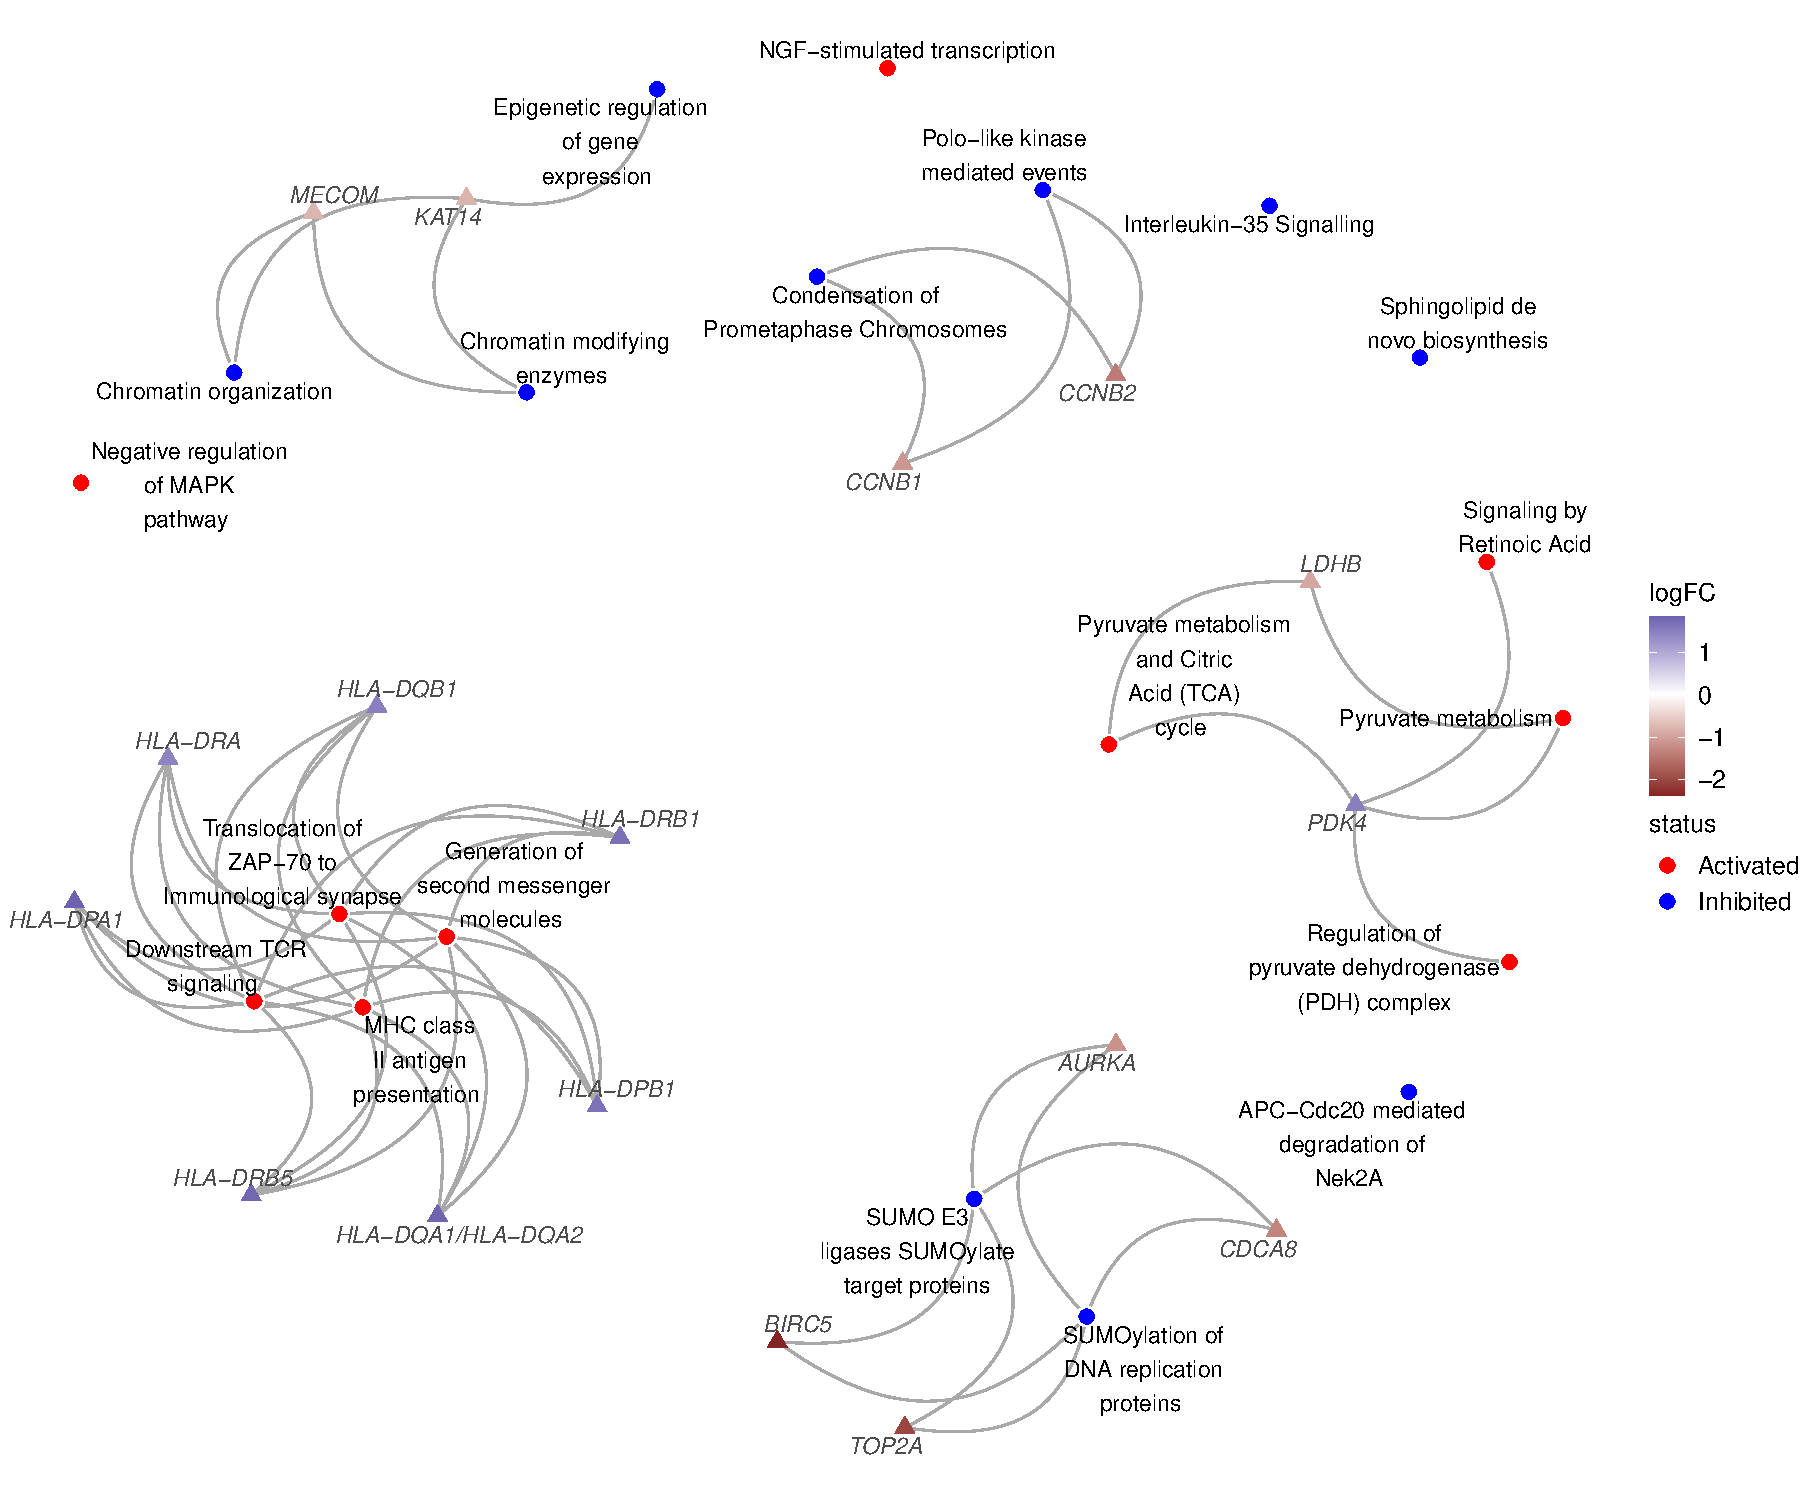
\includegraphics[width=0.8\linewidth]{sSNAPPY_paper_files/figure-latex/Figure6-1} 

}

\caption{Significantly perturbed KEGG pathways identified among post-chemotherapy samples using sSNAPPY, showing any genes in the top 500 ranked for magnitudes of changes in expressions, and which pathways they are likely contributing to. No genes in the top500 were found to contribute to the perturbation of the AMPK signaling pathway or the Toxoplasmosis pathway.}\label{fig:Figure6}
\end{figure}

\hypertarget{identifying-key-gene-contributions}{%
\subsection{Identifying Key Gene Contributions}\label{identifying-key-gene-contributions}}

To further investigate a specific pathway and elucidate the key genes that contribute to its perturbation, we can generate a heatmap via \texttt{plot\_gene\_contribution()} which shows the gene-level perturbation scores for the top-ranked members of a given pathway.
This function takes advantage of the plotting capabilities of the \texttt{pheatmap} package\citep{pheatmap}, and as such, other annotations are also able to be easily included, such as the disease stage, or which general ranges the pathway-level normalised Z-Scores are in.
Inclusion of the Z-Scores enabled the assessment of the level of perturbation predicted in each sample and key genes involved (Figure \ref{fig:Figure7}).

\begin{Shaded}
\begin{Highlighting}[]
\NormalTok{annotation\_df }\OtherTok{\textless{}{-}}\NormalTok{ normalisedScores }\SpecialCharTok{\%\textgreater{}\%}
\NormalTok{    dplyr}\SpecialCharTok{::}\FunctionTok{filter}\NormalTok{(gs\_name }\SpecialCharTok{==} \StringTok{"kegg.p53 signaling pathway"}\NormalTok{) }\SpecialCharTok{\%\textgreater{}\%}
    \FunctionTok{left\_join}\NormalTok{(dplyr}\SpecialCharTok{::}\FunctionTok{select}\NormalTok{(sample\_meta, sample, Stage), }\AttributeTok{by =} \StringTok{"sample"}\NormalTok{) }\SpecialCharTok{\%\textgreater{}\%}
    \FunctionTok{mutate}\NormalTok{(}
      \StringTok{\textasciigrave{}}\AttributeTok{Z Range}\StringTok{\textasciigrave{}} \OtherTok{=} \FunctionTok{cut}\NormalTok{(}
\NormalTok{        robustZ, }\AttributeTok{breaks =} \FunctionTok{seq}\NormalTok{(}\SpecialCharTok{{-}}\DecValTok{2}\NormalTok{, }\DecValTok{2}\NormalTok{, }\AttributeTok{length.out =} \DecValTok{6}\NormalTok{), }\AttributeTok{include.lowest =} \ConstantTok{TRUE}
\NormalTok{      ), }
      \AttributeTok{sample =} \FunctionTok{str\_remove\_all}\NormalTok{(sample, }\StringTok{"\_post{-}NACT"}\NormalTok{)}
\NormalTok{    ) }\SpecialCharTok{\%\textgreater{}\%} 
\NormalTok{    dplyr}\SpecialCharTok{::}\FunctionTok{select}\NormalTok{(sample, }\StringTok{\textasciigrave{}}\AttributeTok{Z Range}\StringTok{\textasciigrave{}}\NormalTok{, Stage)  }
\NormalTok{z\_levels }\OtherTok{\textless{}{-}} \FunctionTok{levels}\NormalTok{(annotation\_df}\SpecialCharTok{$}\StringTok{\textasciigrave{}}\AttributeTok{Z Range}\StringTok{\textasciigrave{}}\NormalTok{)}
\NormalTok{annotation\_col }\OtherTok{\textless{}{-}} \FunctionTok{list}\NormalTok{(}
  \AttributeTok{Stage =} \FunctionTok{c}\NormalTok{(}\AttributeTok{IIIC =} \StringTok{"\#4B0055"}\NormalTok{, }\AttributeTok{IVA =} \StringTok{"\#009B95"}\NormalTok{, }\AttributeTok{IVB =} \StringTok{"\#FDE333"}\NormalTok{),}
  \StringTok{\textasciigrave{}}\AttributeTok{Z Range}\StringTok{\textasciigrave{}} \OtherTok{=} \FunctionTok{setNames}\NormalTok{(}
    \FunctionTok{colorRampPalette}\NormalTok{(}\FunctionTok{c}\NormalTok{(}\StringTok{"navyblue"}\NormalTok{, }\StringTok{"white"}\NormalTok{, }\StringTok{"darkred"}\NormalTok{))(}\FunctionTok{length}\NormalTok{(z\_levels)),}
\NormalTok{    z\_levels}
\NormalTok{  )}
\NormalTok{)}
\FunctionTok{plot\_gene\_contribution}\NormalTok{(}
    \AttributeTok{genePertMatr =}\NormalTok{ genePertScore}\SpecialCharTok{$}\StringTok{\textasciigrave{}}\AttributeTok{kegg.p53 signaling pathway}\StringTok{\textasciigrave{}} \SpecialCharTok{\%\textgreater{}\%}
        \FunctionTok{set\_colnames}\NormalTok{(}\FunctionTok{str\_remove\_all}\NormalTok{(}\FunctionTok{colnames}\NormalTok{(.), }\StringTok{"\_post{-}NACT"}\NormalTok{)),}
    \AttributeTok{color =} \FunctionTok{rev}\NormalTok{(colorspace}\SpecialCharTok{::}\FunctionTok{divergex\_hcl}\NormalTok{(}\DecValTok{100}\NormalTok{, }\AttributeTok{palette =} \StringTok{"RdBu"}\NormalTok{)),}
    \AttributeTok{breaks =} \FunctionTok{seq}\NormalTok{(}\SpecialCharTok{{-}}\FloatTok{0.0015}\NormalTok{, }\FloatTok{0.0015}\NormalTok{, }\AttributeTok{length.out =} \DecValTok{100}\NormalTok{), }
    \AttributeTok{annotation\_df =}\NormalTok{  annotation\_df, }
    \AttributeTok{topGene =} \DecValTok{20}\NormalTok{, }\AttributeTok{filterBy =} \StringTok{"mean"}\NormalTok{, }
    \AttributeTok{mapEntrezID =}\NormalTok{ entrez2name,}
    \AttributeTok{annotation\_colors =}\NormalTok{ annotation\_col,}
    \AttributeTok{cutree\_rows =} \DecValTok{3}\NormalTok{, }\AttributeTok{cutree\_cols =} \DecValTok{3}\NormalTok{,}
    \AttributeTok{main =} \StringTok{"P53 Signaling Pathway [KEGG]"}
\NormalTok{)}
\end{Highlighting}
\end{Shaded}

\begin{figure}

{\centering 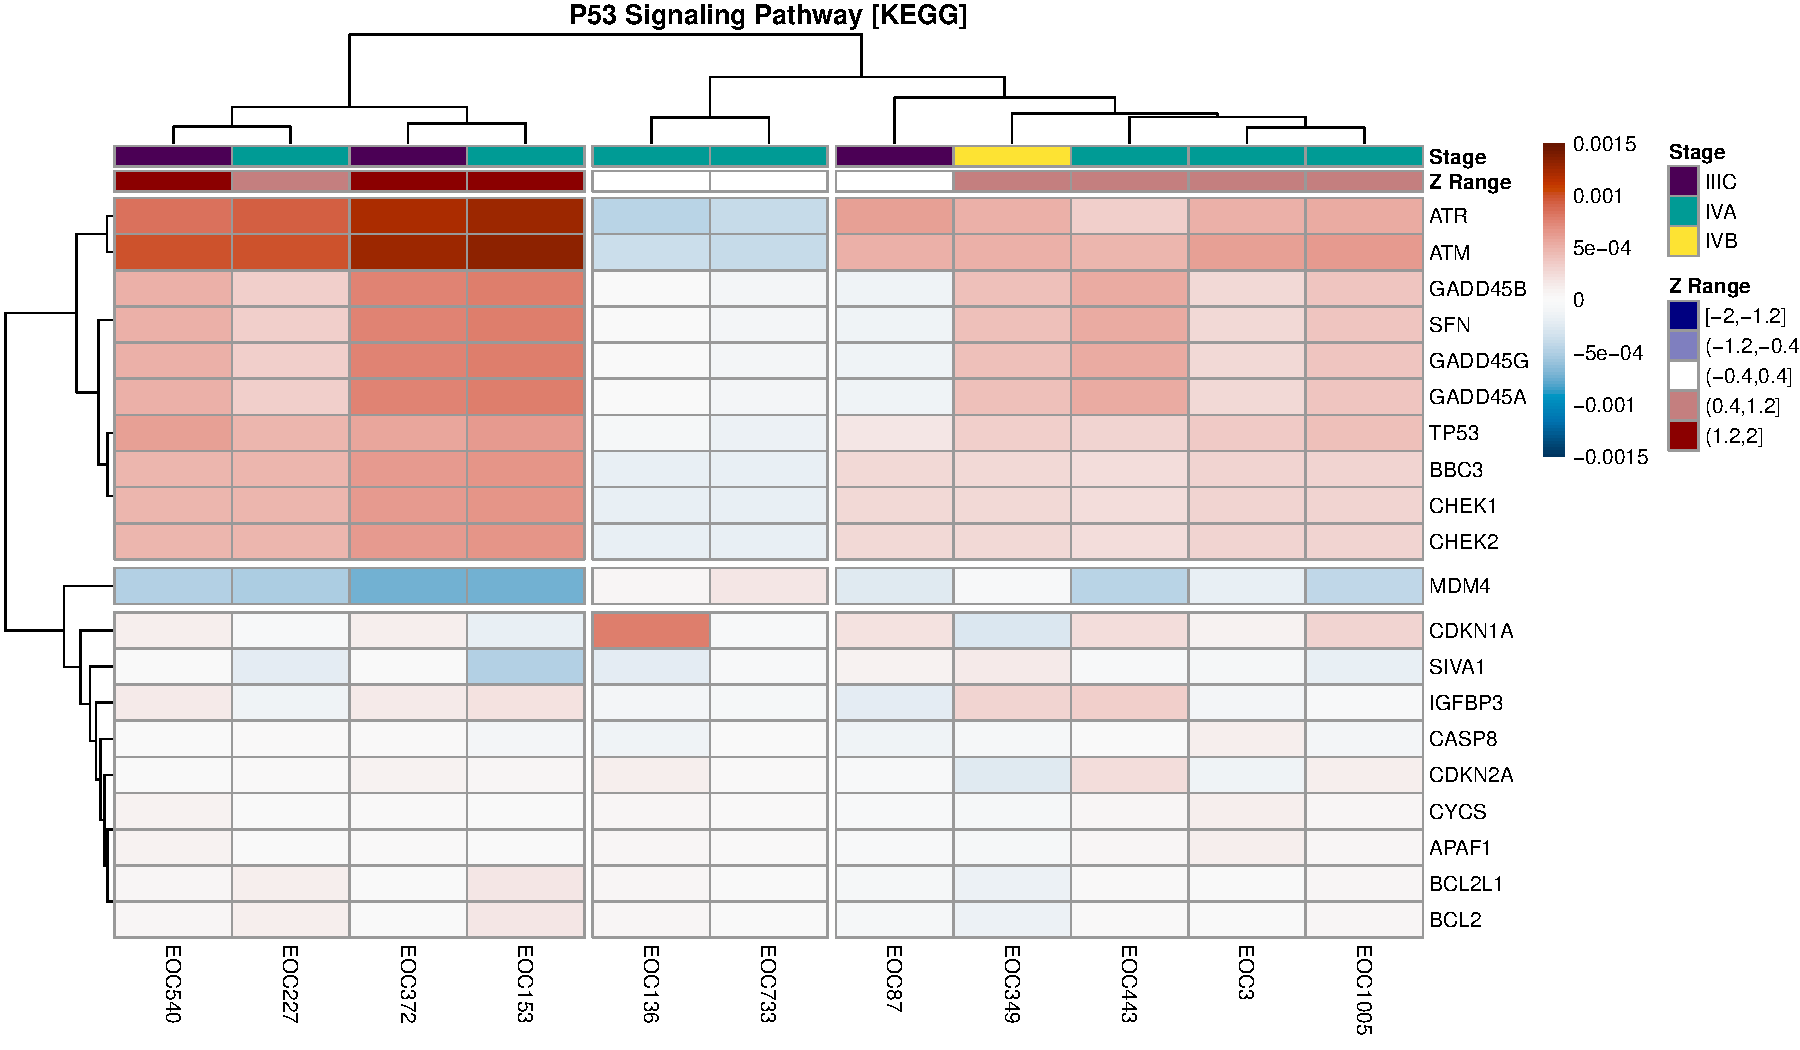
\includegraphics[width=1\linewidth]{sSNAPPY_paper_files/figure-latex/Figure7-1} 

}

\caption{Gene-level perturbation scores of the top 20 genes in the "p53 signalling pathway" ranked by their average contribution to the perturbation score. Samples were annotated by the stage of cancers, along with robust Z-scores which indicate the extent of perturbation within each sample. The genes ATR and ATM were identified as possible key drivers of the activation of p53 signalling pathway, with downregulation of MDM4 also appearing likely to be playing a role.}\label{fig:Figure7}
\end{figure}

From this heatmap we can identify candidate genes which are likely to be making the biggest contribution to the activation of p53 Signaling Pathway upon chemotherapy, such as \emph{ART} and \emph{ATM}, along with the \emph{MDM4} and members of the GADD45 family.
Ataxia-telangiectasia mutated (\emph{ATM}) is a well-established oncosuppressor\citep{Moslemi2021} while haploinsufficient mouse double minute 4 (\emph{MDM4}) is an oncogene that suppresses p53\citep{Momand}. Mutations of both genes have been observed in many types of cancers\citep{Choi2016, Gansmo2016, Atwal2009}.
Moreover, the Ataxia telangiectasia and RAD3-related protein kinase (\emph{ATR}) and the growth arrest and DNA damage-inducible gene 45 (\emph{GADD45}) have gained great attention as potential targets for anti-tumor treatments due to their involvement in DNA damage repair\citep{Liebermann2011, Hu2022}.
ATR inhibitors, in particular, have shown promising results in clinical trials for HGSOC.\citep{Li2022, Gong2021}.

\hypertarget{discussion}{%
\section{Discussion}\label{discussion}}

In conclusion, we have presented and provided a demonstration for the R/Bioconductor package \emph{sSNAPPY} which offers a novel single-sample pathway perturbation testing approach, tailored for heterogeneous tissue samples in matched-pair design.
In contrast to many common enrichment methods, sSNAPPY uses pathway topology information to compute perturbation scores which indicate the likely impact on the activity of a pathway, by predicting direction of change.
By applying sSNAPPY to a public scRNA-seq data collected before and after HGSOC patients were subjected to chemotherapy, we demonstrated its ability to detect significant pathway perturbations of various interesting biological processes consistent with, and far beyond what was shown in the original study.
\emph{sSNAPPY} addresses the limitations of alternative strategies that fail to account for gene-gene interactions encoded by pathway topologies or predict the directionality of pathway activities.
In addition, the single-sample nature of the method can be utilised to address the increasing demand for personalised medicine.
Through identifying shared and divergent responses between individuals, \emph{sSNAPPY} can provide valuable insights into the heterogeneous responses across clinical samples.
Overall, we believe sSNAPPY represents a valuable addition to the existing body of pathway analysis methods.

\hypertarget{data-availability}{%
\section{Data availability}\label{data-availability}}

The dataset analysed in this manuscript are stored in the data directory of this GitHub repository.

\hypertarget{software-availability}{%
\section{Software availability}\label{software-availability}}

\begin{itemize}
\item
  Software available from: \url{https://bioconductor.org/packages/release/bioc/html/sSNAPPY.html}
\item
  Source code available from: \url{https://github.com/Wenjun-Liu/sSNAPPY}
\item
  Archived source code at time of publication: {[}DOI (found on right hand side of a Zenodo record){]}
\item
  License: \href{https://opensource.org/license/mit/}{MIT}
\end{itemize}

\hypertarget{competing-interests}{%
\section{Competing interests}\label{competing-interests}}

No competing interests were disclosed

\hypertarget{grant-information}{%
\section{Grant information}\label{grant-information}}

This work was supported by funding from the National Health and Medical Research Council of Australia (ID 1186647 to W.D. Tilley) and the National Breast Cancer Foundation Australia (ID IIRS-23-069 to W.D. Tilley).

\hypertarget{acknowledgements}{%
\section{Acknowledgements}\label{acknowledgements}}

\renewcommand\refname{References}
{\small\bibliography{sample.bib}}

\end{document}
